\documentclass[a4paper]{wmpart}

\usepackage{tgtermes}
\usepackage[T1]{fontenc}
\usepackage{polski}
\usepackage[utf8]{inputenc}
\input{glyphtounicode}
\pdfgentounicode=1
\usepackage{amsthm}
\usepackage[colorlinks]{hyperref}
\usepackage{tikz}
\usepackage{graphicx}
\usepackage{microtype}
\usetikzlibrary{cd}
\usetikzlibrary{babel}
\nonfrenchspacing

% Makra i definicje środowisk

%% Przykłady komend bez argumentów:
\newcommand{\mlr}{\leqslant} %% skrót na symbol "mniejsze lub równe"
\newcommand{\wlr}{\geqslant} %% skrót na symbol "większe lub równe"
\newcommand{\diam}{\operatorname{diam}}
\newcommand{\dist}{\operatorname{dist}}
\newcommand{\R}{\mathbb{R}} %% zbiór liczb rzeczywistych
\newcommand{\N}{\mathbb{N}} %% zbiór liczb naturalnych
\newcommand{\Z}{\mathbb{Z}} %% zbiór liczb całkowitych
\newcommand{\Q}{\mathbb{Q}} %% zbiór liczb wymiernych
\newcommand{\C}{\mathbb{C}} %% zbiór liczb zespolonych
\newcommand{\Real}[1]{\R^{#1}}
\newcommand{\Rn}{\Real{n}}
\newcommand{\Borel}[1]{\mathcal{B}({#1})}
\newcommand{\BorelRn}{\Borel{\Rn}}
\newcommand{\BorelR}{\Borel{\R}}
\newcommand{\Leb}[1]{\mathcal{L}({#1})}

\newcommand{\sequence}[1]{\left({#1}_n\right)_{n\in\N}} %% ciąg nieskończony
\newcommand{\seqlim}[1]{\lim\limits_{n\to\infty}{#1}_n}
\newcommand{\pair}[2]{\left\langle {#1}, {#2} \right\rangle} %% para uporzadkowana
\newcommand{\subs}{\subseteq } % inkluzja
\newcommand{\sups}{\supseteq} % odwrócona inkluzja
\newcommand{\setof}[2]{\left\{#1 \colon #2 \right\}} % zbiór postaci { ... : ... }
\renewcommand{\Im}{\operatorname{Im}} % Domyślnie \Im to gotyckie I (część rzeczywista liczby)
\renewcommand{\Re}{\operatorname{Re}} % Domyślnie \Re to gotyckie R (część urojona liczny)
\newcommand{\fun}[3]{#1 \colon #2 \to #3}
\newcommand{\eps}{\varepsilon} % Może być też \epsilon, ale wygląda to trochę dziwnie.
\newcommand{\separator}{\begin{center}***\end{center}} % Trzy gwiazdki oddzielające paragrafy

% Środowiska twierdzeniowe
\newtheorem{tw}{Twierdzenie}[section]
\newtheorem{lem}[tw]{Lemat}
\newtheorem{wn}[tw]{Wniosek}
\theoremstyle{definition}
\newtheorem{defi}[tw]{Definicja}
\newtheorem{uwaga}[tw]{Uwaga}
\newtheorem{fakt}[tw]{Fakt}

\renewcommand\thetw{\thesection.\arabic{tw}}
\renewcommand\thedefi{\thesection.\arabic{defi}}
\renewcommand\theuwaga{\thesection.\arabic{uwaga}}
\renewcommand\thetw{\thesection.\arabic{tw}}
\renewcommand\thelem{\thesection.\arabic{lem}}
\renewcommand\thewn{\thesection.\arabic{wn}}

\newenvironment{dow}{\begin{proof}[\textbf{Dowód}]}{\end{proof}} 


\bibliographystyle{plain}

\uczelnia{Uniwersytet Kardynała Stefana Wyszyńskiego w~Warszawie}
\instytut{Wydział Matematyczno-Przyrodniczy. Szkoła Nauk Ścisłych}
%autor pracy:
\author{Tomasz Perek}
%numer albumu:
\nralbumu{128883}

\title{Konstrukcja miary Lebesgue'a w $\Rn$. Charakteryzacja zbiorów mierzalnych w sensie Lebesgue'a i własności miary Lebesgue'a}
\kierunek{matematyka zaoczna}

\date{2026}
\keywords{miara Lebesgue'a, miara zewnętrzna, warunek Carathéodory'ego, zbiory borelowskie, regularność miary, zbiór Vitalego, niezmienniczość na translacje}


\begin{document}

\maketitle

\begin{abstract}
    Niniejsza praca poświęcona jest systematycznemu przedstawieniu miary Lebesgue'a w przestrzeni euklidesowej $\Rn$. Wychodząc od elementarnego pojęcia objętości $n$-wymiarowych kostek, konstruuje się zewnętrzną miarę Lebesgue'a, a następnie za pomocą metody Carathéodory'ego wyznacza się $\sigma$-algebrę zbiorów mierzalnych w sensie Lebesgue'a. Szczególną uwagę poświęcono charakteryzacji zbiorów mierzalnych w sensie Lebesgue'a oraz własnościom samej miary.
\end{abstract}



\tableofcontents


\section{Wstęp}
Miara Lebesgue'a, czyli miara podzbiorów przestrzeni rzeczywistej $\R$ (i ogólniej, $\Rn$), pochodzi z pracy Henriego Lebesgue'a, która dotyczyła rozszerzenia pojęcia całki na znacznie szerszą klasę funkcji niż całka Riemanna (tzw. całka Lebesgue'a). Teoria miary niemal od początku stawiała pytanie, czy istnieje miara, czyli funkcja przypisująca podzbiorom ustalonego zbioru nieujemne wartości liczbowe lub $+\infty$ w taki sposób, że zbiór pusty ma miarę zero, a miara sumy przeliczalnej rodziny parami rozłącznych zbiorów jest równa sumie ich miar, która ponadto (1) jest określona na wszystkich podzbiorach $\R$, (2) jest niezmiennicza na przesunięcia oraz (3) przypisuje przedziałowi jednostkowemu wartość 1. W teorii zbiorów z aksjomatem wyboru taka miara nie istnieje. Miara Lebesgue'a spełnia drugi i trzeci z tych warunków, a zamiast pierwszego podaje kryterium, które dzieli wszystkie podzbiory zbioru liczb rzeczywistych na mierzalne oraz niemierzalne. Definicja miary Lebesgue'a $\lambda$ opiera się na definicji miary zewnętrznej Lebesgue'a $\lambda^{*}$, która jest określona na zbiorze wszystkich podzbiorów przestrzeni $\Rn$. Miara zewnętrzna Lebesgue'a jest niezmiennicza na przesunięcia oraz kostce jednostkowej przypisuje wartość 1, co znaczy, że jest odpowiednia do pomiaru wielkości geometrycznych, takich jak długość, pole powierzchni czy objętość. Nie jest ona jednak przeliczalnie addytywna, co oznacza, że miara sumy zbiorów rozłącznych może być mniejsza niż suma miar tych zbiorów. Właściwa miara Lebesgue'a nie ma już tej wady (tzn.\ jest przeliczalnie addytywna): jest równa mierze zewnętrznej Lebesgue'a, ale jej dziedzina jest ograniczona do zbiorów spełniających warunek Carathéodory'ego; zbiory te tworzą $\sigma$-ciało, które jest dziedziną miary Lebesgue'a. W pracy tej odtwarza się krok po kroku proces wiodący do konstrukcji tej miary.

\section{Podstawowe pojęcia}
Zanim przystąpimy do konstrukcji narzędzi mierzących skomplikowane zbiory, musimy precyzyjnie określić środowisko, w którym będziemy operować. Nie możemy oczekiwać, że każda dowolna rodzina podzbiorów zachowa się stabilnie przy operacjach sumowania czy dopełniania. W niniejszym rozdziale wprowadzamy zatem algebraiczny szkielet teorii — od pierścieni i ciał, przez kluczowe pojęcie $\sigma$-algebry, aż po topologię euklidesową przestrzeni $\Rn$, która wyznaczy geometryczny punkt odniesienia dla pojęcia objętości.

\subsection{Struktury rodzin zbiorów}
W poniższych definicjach niech $X$ będzie ustalonym niepustym zbiorem.
\begin{defi}[Pierścień zbiorów]
    \textbf{Pierścieniem podzbiorów} przestrzeni $X$ nazywamy rodzinę $\mathcal{R} \subs \mathcal{P}(X)$, zawierającą $\emptyset$, zamkniętą na skończone sumy i różnice zbiorów, tj. spełniającą warunki:
    \begin{enumerate}
        \item $\emptyset \in \mathcal{R}$
        \item $\forall_{A, B \in \mathcal{R}} A \cup B \in \mathcal{R}$
        \item $\forall_{A, B \in \mathcal{R}} A \setminus B \in \mathcal{R}$
    \end{enumerate}
\end{defi}

\begin{defi}[Algebra (ciało) zbiorów]
    \textbf{Algebrą (bądź ciałem)} podzbiorów przestrzeni $X$  nazywamy pierścień $\mathcal{F}$ podzbiorów $X$, zawierający całą przestrzeń $X$. Równoważnie, algebrę podzbiorów przestrzeni $X$ możemy zdefiniować jako rodzinę $\mathcal{F}$ podzbiorów przestrzeni $X$ spełniającą następujące warunki:
    \begin{enumerate}
        \item $\emptyset \in \mathcal{F}$
        \item $\forall_{A,B \in \mathcal{F}} A \cup B \in \mathcal{F}$
        \item $\forall_{A \in \mathcal{F}} X \setminus A \in \mathcal{F}$
    \end{enumerate}
\end{defi}

\begin{defi}[$\sigma$-algebra ($\sigma$-ciało)]
    \textbf{$\sigma$-ciałem (lub przeliczalnie addytywnym ciałem)} podzbiorów przestrzeni $X$ nazywamy rodzinę $\mathcal{M}$ podzbiorów $X$ spełniającą następujące warunki:
    \begin{enumerate}
        \item $\emptyset \in \mathcal{M}$
        \item $\forall_{A \in \mathcal{M}} X \setminus A \in \mathcal{M}$
        \item $\forall_{A_1, A_2, \ldots \in \mathcal{M}} \bigcup_{n = 1}^\infty A_n \in \mathcal{M}$
    \end{enumerate}
    Parę $(X, \mathcal{M})$ nazywamy \textbf{przestrzenią mierzalną}, a zbiory należące do rodziny $\mathcal{M}$ zbiorami $\mathcal{M}$-mierzalnymi (lub mierzalnymi).
    $\sigma$-algebra podzbiorów przestrzeni $X$ jest więc algebrą w której ,,warunek sumy'' rozszerzono na sumę przeliczalnej rodziny zbiorów. W oczywisty sposób każda $\sigma$-algebra jest algebrą, choć odwrotne twierdzenie nie zawsze jest prawdziwe.
\end{defi}

\begin{defi}[$\sigma$-algebra generowana]
    $\sigma$-algebrą generowaną przez rodzinę zbiorów $\mathcal{F}$ nazywamy najmniejszą $\sigma$-algebrę zawierającą tę rodzinę i oznaczamy $\sigma(\mathcal{F})$.
\end{defi}

\subsection{Elementarna geometria i topologia w $\Rn$}

W całej pracy przestrzeń $\Rn$ ($n \in \N$, $n \wlr 1$) traktujemy jako $n$-wymiarową przestrzeń liniową nad ciałem liczb rzeczywistych $\R$. Punkty przestrzeni oznaczamy przez $x = (x_1, \ldots, x_n)$, $y = (y_1, \ldots, y_n) \in \Rn$.

\begin{defi}[Metryka i topologia euklidesowa]
    Dla dowolnych punktów $x, y \in \Rn$ \textbf{odległością euklidesową} (metryką euklidesową) nazywamy liczbę
    \begin{equation*}
        d(x, y) = \|x - y\| = \sqrt{\sum_{i=1}^n (x_i - y_i)^2}.
    \end{equation*}
    \begin{enumerate}
        \item \textbf{Kulą otwartą} o środku w punkcie $x_0 \in \Rn$ i promieniu $r > 0$ nazywamy zbiór
              \begin{equation*}
                  B(x_0, r) := \setof{x \in \Rn}{d(x, x_0) < r}
              \end{equation*}

        \item Zbiór $U \subseteq  \Rn$ nazywamy \textbf{zbiorem otwartym}, jeżeli dla każdego $x \in U$ istnieje $r > 0$ takie, że $B(x, r) \subseteq  U$.
              Rodzinę wszystkich zbiorów otwartych w $\Rn$ oznaczamy przez $\mathrm{top}(\Rn)$.

        \item Zbiór $F \subseteq  \Rn$ nazywamy \textbf{zbiorem domkniętym}, jeżeli jego dopełnienie $F^c = \Rn \setminus F$ jest zbiorem otwartym ($F^c \in \mathrm{top}(\Rn)$).
              Rodzinę wszystkich zbiorów domkniętych oznaczamy przez $\mathrm{cotop}(\Rn)$.

        \item Zbiór $K \subseteq  \Rn$ nazywamy \textbf{zbiorem zwartym}, jeżeli z każdego jego pokrycia zbiorami otwartymi można wybrać podpokrycie skończone. Na mocy twierdzenia Heinego-Borela zbiór $K \subseteq  \Rn$ jest zwarty wtedy i tylko wtedy, gdy jest domknięty i ograniczony w metryce euklidesowej.

        \item Dla dowolnego niepustego zbioru $A \subseteq \Rn$ liczbę
              \begin{equation*}
                  \diam(A) := \sup\setof{d(x, y)}{x, y \in A} \in [0, +\infty]
              \end{equation*} nazywamy \textbf{średnicą zbioru} $A$. Przyjmujemy ponadto $\diam(\emptyset) = 0$.
        \item Dla dwóch niepustych podzbiorów $A, B \subseteq \Rn$ \textbf{odległością zbiorów} $A$ i $B$ nazywamy wielkość
              \begin{equation*}
                  \dist(A, B) := \inf\setof{d(x, y)}{x \in A,  y \in B}.
              \end{equation*}
              Przyjmujemy $\dist(A, B) = +\infty$, gdy $A = \emptyset$ lub $B = \emptyset$. Dla punktu $x \in \Rn$ piszemy $\dist(x, A) := \dist(\{x\}, A)$.
    \end{enumerate}
\end{defi}

\begin{defi}[Kostka w $\Rn$]
    Niech $a_j, b_j \in \R$ spełniają $a_j < b_j$ dla każdego $j \in \{1, \ldots, n\}$.

    \begin{enumerate}
        \item \textbf{Kostką domkniętą} (przedziałem wielowymiarowym domkniętym) w $\Rn$ nazywamy iloczyn kartezjański odcinków domkniętych:
              \begin{equation*} P = [a_1, b_1] \times [a_2, b_2] \times \ldots \times [a_n, b_n] = \prod_{j=1}^n [a_j, b_j].
              \end{equation*}
        \item \textbf{Kostką otwartą} w $\Rn$ nazywamy zbiór postaci:
              \begin{equation*} Q = (a_1, b_1) \times (a_2, b_2) \times \ldots \times (a_n, b_n) = \prod_{j=1}^n (a_j, b_j).
              \end{equation*}
        \item Ogólnie, \textbf{kostką ograniczoną} (przedziałem $n$-wymiarowym) w $\Rn$ nazywamy zbiór będący iloczynem kartezjańskim dowolnych przedziałów jednowymiarowych o końcach $a_j, b_j$ (domkniętych, otwartych lub jednostronnie domkniętych). Każda taka kostka $R$ spełnia relację $Q \subseteq  R \subseteq  P$ dla odpowiednich kostek otwartej $Q$ i domkniętej $P$.
    \end{enumerate}
\end{defi}

\begin{defi}[Elementarna objętość kostki] Dla dowolnej ograniczonej kostki $R \subseteq \Rn$ (domkniętej, otwartej bądź częściowo domkniętej) o końcach odcinków krawędziowych $a_j < b_j$ ($j = 1, \ldots, n$) definiujemy jej \textbf{objętość elementarną} wzorem:
    \begin{equation*}
        V^n(R) := \prod_{j=1}^n (b_j - a_j).
    \end{equation*}
    Ponadto dla zbioru pustego kładziemy $V^n(\emptyset) := 0$.
\end{defi}

\begin{defi}[$\sigma$-algebra zbiorów borelowskich]
    Niech $\mathrm{top}(\Rn)$ oznacza rodzinę wszystkich podzbiorów otwartych w $\Rn$. $\sigma$-algebrę generowaną przez tę rodzinę, oznaczaną symbolem $\BorelRn$, nazywamy \textbf{$\sigma$-algebrą zbiorów borelowskich} w $\Rn$:
    \begin{equation*}
        \Borel{\Rn} := \sigma(\mathrm{top}(\Rn)).
    \end{equation*}
    Elementy rodziny $\BorelRn$ nazywamy \textbf{zbiorami borelowskimi}.
\end{defi}
\begin{uwaga}
    Zauważmy, że ponieważ dopełnienie zbioru otwartego jest zbiorem domkniętym, zachodzi tożsamość: \begin{equation*} \BorelRn = \sigma(\mathrm{cotop}(\Rn)).
    \end{equation*}
    Co więcej, $\sigma$-algebra $\BorelRn$ jest generowana przez każdą z poniższych rodzin:
    \begin{enumerate}
        \item rodzinę wszystkich kostek otwartych w $\Rn$;
        \item rodzinę wszystkich kostek domkniętych w $\Rn$;
        \item rodzinę kostek postaci $\prod_{j=1}^n [a_j, b_j)$ lub $\prod_{j=1}^n (a_j, b_j)$ o końcach wymiernych $a_j, b_j \in \Q$.
    \end{enumerate}
\end{uwaga}
\begin{defi}[Klasy borelowskie $G_\delta$ oraz $F_\sigma$]
    Niech $Y \subseteq  \Rn$.
    \begin{enumerate}
        \item Zbiór $Y$ nazywamy \textbf{zbiorem typu $G_\delta$}, jeżeli jest on przeliczalnym przekrojem zbiorów otwartych, to znaczy:
              \begin{equation*}
                  \exists \{G_j\}_{j=1}^\infty \subseteq  \mathrm{top}(\Rn) \quad \text{taki, że} \quad Y = \bigcap_{j=1}^\infty G_j.
              \end{equation*}
        \item Zbiór $Y$ nazywamy \textbf{zbiorem typu $F_\sigma$}, jeżeli jest on przeliczalną sumą zbiorów domkniętych, to znaczy:
              \begin{equation*}
                  \exists \, \{F_j\}_{j=1}^\infty \subseteq  \mathrm{cotop}(\Rn) \quad \text{taki, że} \quad Y = \bigcup_{j=1}^\infty F_j.
              \end{equation*}
    \end{enumerate}
\end{defi}
\begin{wn} W przestrzeni euklidesowej $\Rn$ (i ogólniej w dowolnej przestrzeni metrycznej):
    \begin{enumerate}
        \item Każdy zbiór domknięty jest typu $G_\delta$, tj. $\mathrm{cotop}(\Rn) \subseteq  G_\delta$.
        \item Każdy zbiór otwarty jest typu $F_\sigma$, tj. $\mathrm{top}(\Rn) \subseteq  F_\sigma$.
        \item Wszystkie zbiory klas $G_\delta$ oraz $F_\sigma$ są zbiorami borelowskimi ($G_\delta \subseteq  \BorelRn$ oraz $F_\sigma \subseteq  \BorelRn$).
    \end{enumerate}
\end{wn}

\section{Zewnętrzna miara Lebesgue'a w $\Rn$}

Objętość elementarna prostopadłościanów jest intuicyjna i jednoznaczna, jednak jej zasięg ogranicza się do najprostszych figur geometrycznych. Naturalnym pytaniem jest: jak przenieść to pojęcie na dowolne, nawet skrajnie nieregularne podzbiory $\Rn$? Klasyczna próba Jordana — polegająca na przybliżaniu zbiorów skończoną liczbą kostek — okazała się zbyt ciasna, uniemożliwiając zmierzenie choćby zbioru liczb wymiernych. Odpowiedzią Lebesgue'a było dopuszczenie przeliczalnych pokryć kostkami. W ten sposób rodzi się zewnętrzna miara Lebesgue'a $\lambda^{*n}$, która potrafi przypisać wielkość każdemu podzbiorowi przestrzeni, choć ceną za tę uniwersalność jest utrata pełnej addytywności.

\subsection{Pojęcie miary zewnętrznej}

\begin{defi}[Miara zewnętrzna]
    Niech $X$ będzie zbiorem niepustym. Funkcję $\phi \colon \mathcal{P}(X) \to [0, +\infty]$ nazywamy \textbf{miarą zewnętrzną} (w sensie Carathéodory'ego) na $X$, jeżeli spełnia następujące warunki:
    \begin{enumerate}
        \item[(i)] $\phi(\emptyset) = 0$;
        \item[(ii)] \textbf{monotoniczność}: jeżeli $A \subseteq  B \subseteq  X$, to $\phi(A) \mlr \phi(B)$;
        \item[(iii)] \textbf{przeliczalna podaddytywność (subaddytywność)}: dla dowolnego przeliczalnego ciągu podzbiorów $\{A_j\}_{j=1}^\infty \subseteq \mathcal{P}(X)$ zachodzi
              \begin{equation*}
                  \phi\left(\bigcup_{j=1}^\infty A_j\right) \mlr \sum_{j=1}^\infty \phi(A_j).
              \end{equation*}
    \end{enumerate}
\end{defi}

\subsection{Definicja zewnętrznej miary Lebesgue'a} Zewnętrzną miarę Lebesgue'a otrzymujemy, przybliżając zbiór z zewnątrz przeliczalnymi pokryciami kostkami i sumując ich objętości elementarne $V^n$.
\begin{defi}[Zewnętrzna miara Lebesgue'a]
    Dla dowolnego zbioru $A \subseteq \Rn$ jego \textbf{zewnętrzną miarą Lebesgue'a} nazywamy liczbę
    \begin{equation*}
        \lambda^{*n}(A) := \inf \left\{ \sum_{j=1}^\infty V^n(P_j) \colon P_j \text{ są kostkami domkniętymi w } \Rn, \; A \subseteq \bigcup_{j=1}^\infty P_j \right\}.
    \end{equation*}
    W literaturze miarę tę oznacza się również przez $L_e^n(A)$.
\end{defi}


\begin{figure}
    \centering
    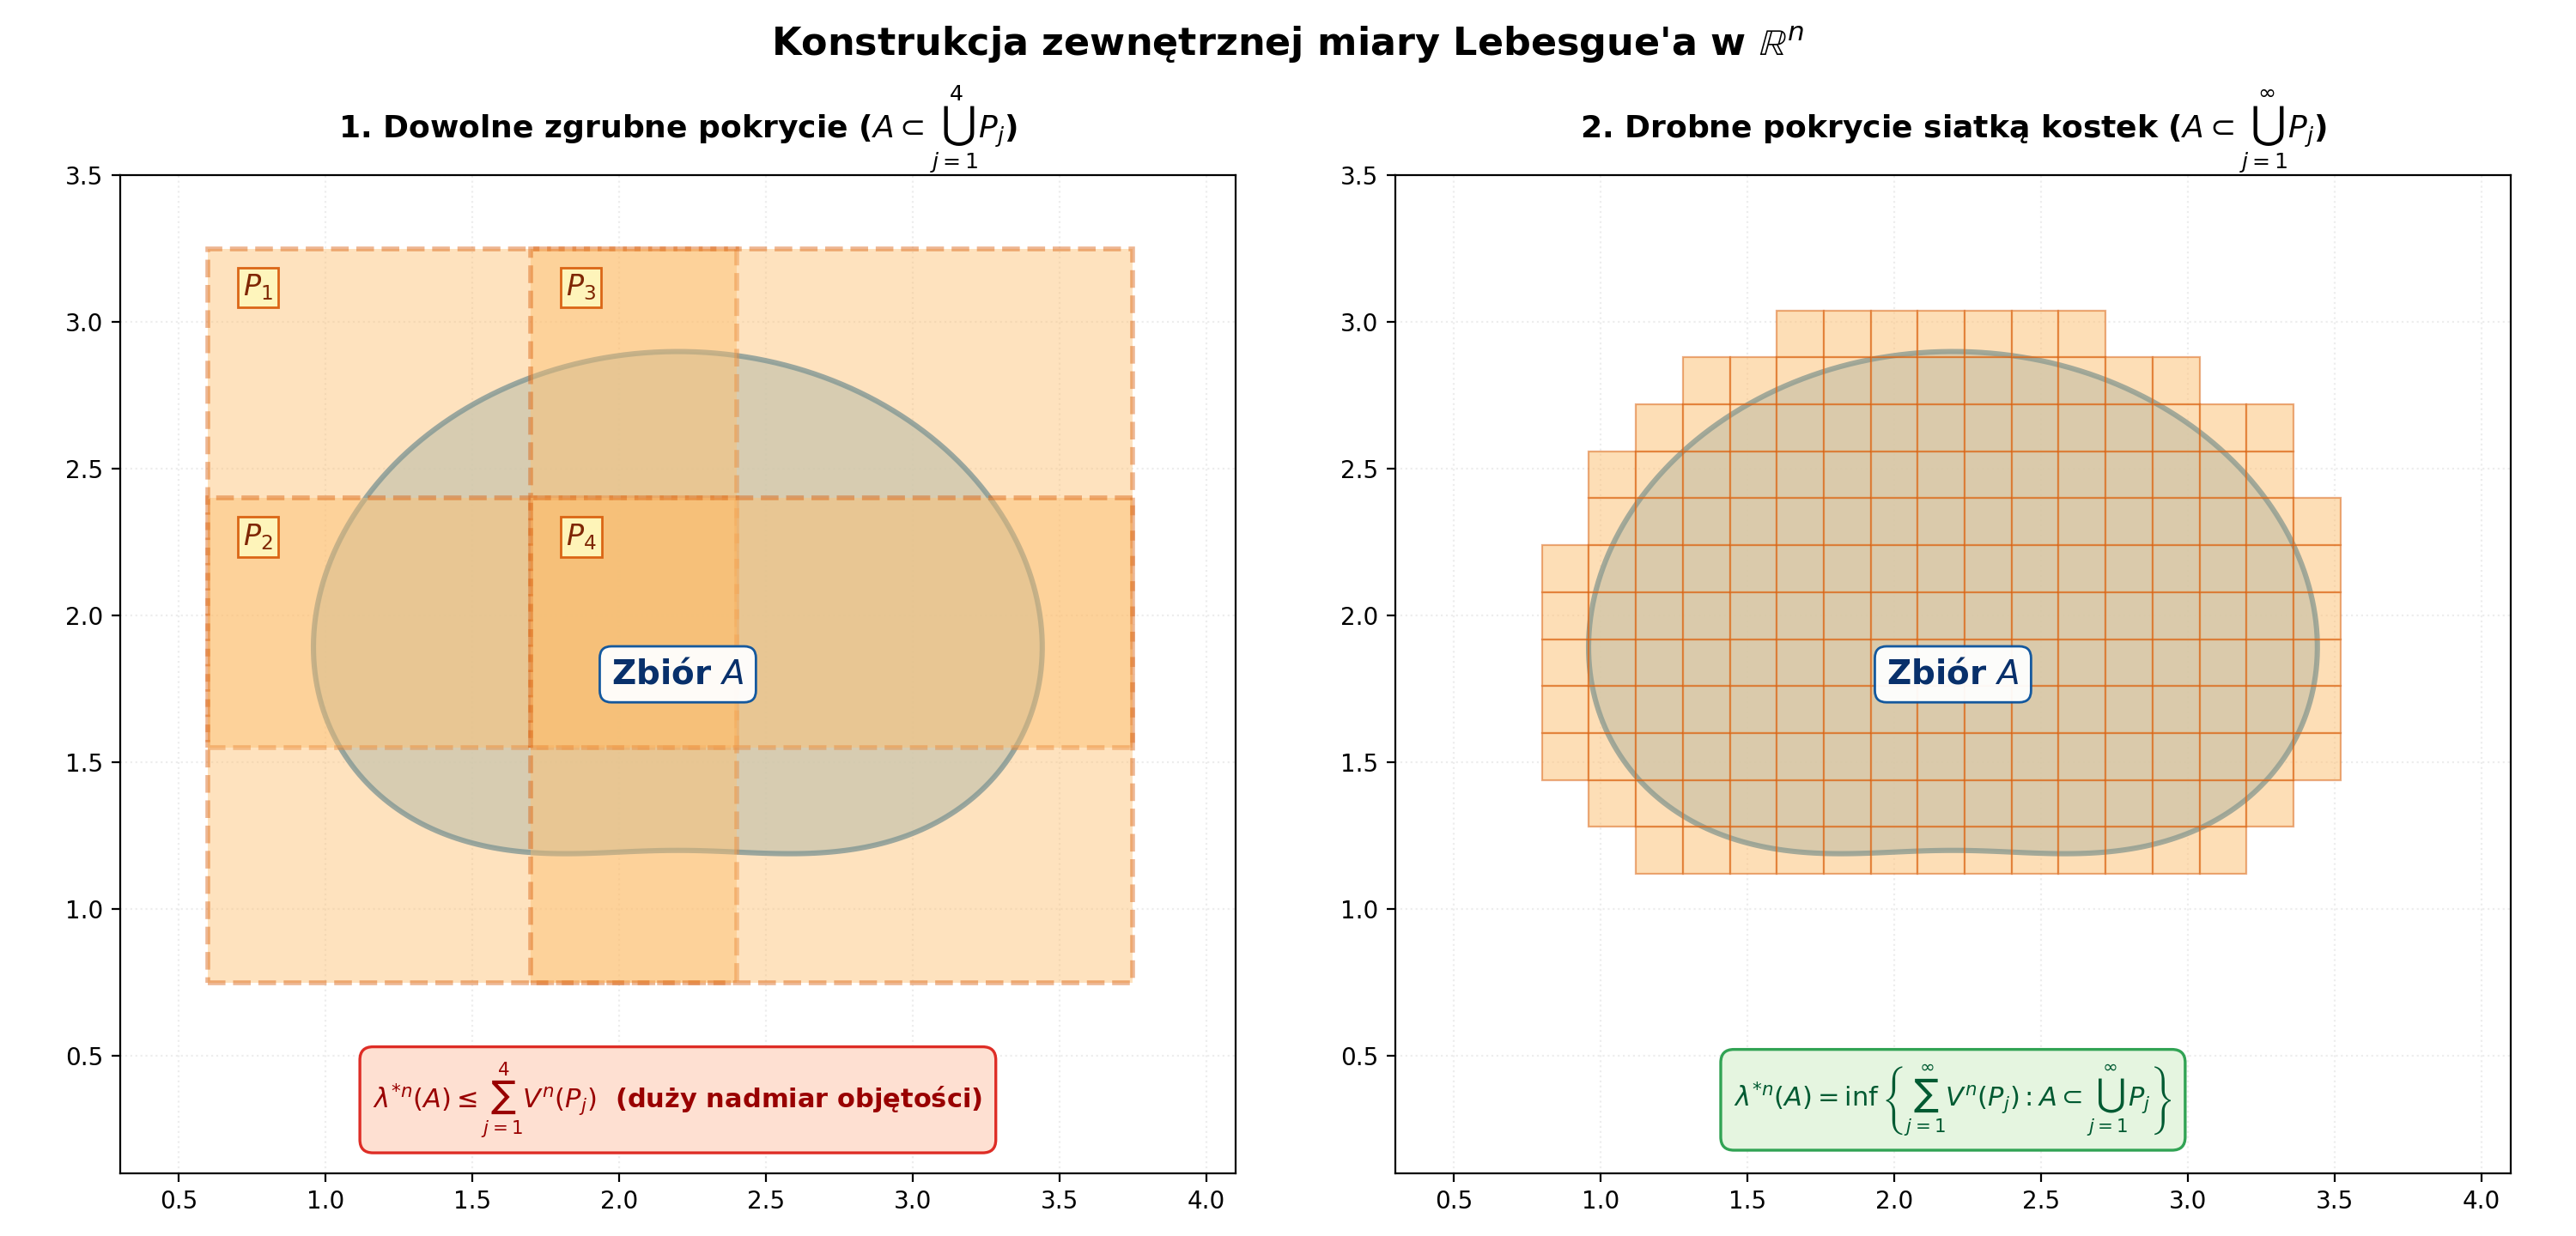
\includegraphics[width=0.5\linewidth]{miara_zewnetrzna_v4.png}
    \caption{Idea konstrukcji zewnętrznej miary Lebesgue'a $\lambda^{*n}(A)$ w $\Rn$: zgrubne pokrycie kostkami z nadmiarem (po lewej) oraz minimalizacja sumy objętości poprzez infimum po coraz drobniejszych pokryciach (po prawej).}
    \label{fig:miara_zewnetrzna}
\end{figure}

\begin{uwaga}[Równoważne warianty pokryć]\label{uwaga:pokrycia} W definicji zewnętrznej miary Lebesgue'a wartość $\lambda^{*n}(A)$ nie ulega zmianie, jeżeli:
    \begin{enumerate}
        \item zamiast kostek domkniętych użyjemy kostek otwartych:
              \begin{equation*} \lambda^{*n}(A) = \inf \left\{ \sum_{j=1}^\infty V^n(Q_j) \colon Q_j \text{ są kostkami otwartymi, } A \subseteq \bigcup_{j=1}^\infty Q_j \right\};
              \end{equation*}
        \item ograniczymy się do kostek (otwartych lub domkniętych) o średnicach mniejszych od ustalonej stałej $\delta > 0$, tj. $\diam(P_j) < \delta$.
    \end{enumerate}
\end{uwaga}
\begin{dow}[Uzasadnienie równoważności pokryć otwartych] Niech $\lambda^{*n}_{\mathrm{open}}(A)$ oznacza infimum po pokryciach kostkami otwartymi. Ponieważ dla każdej kostki otwartej $Q$ jej domknięcie $\overline{Q}$ jest kostką domkniętą o tej samej objętości ($V^n(\overline{Q}) = V^n(Q)$), każde pokrycie kostkami otwartymi generuje dopuszczalne pokrycie kostkami domkniętymi, skąd $\lambda^{*n}(A) \mlr \lambda^{*n}_{\mathrm{open}}(A)$.
    W drugą stronę: niech $\{P_j\}_{j=1}^\infty$ będzie pokryciem zbioru $A$ kostkami domkniętymi takim, że
    \begin{equation*}
        \sum_{j=1}^\infty V^n(P_j) \mlr \lambda^{*n}(A) + \frac{\varepsilon}{2}.
    \end{equation*}
    Dla każdego $j \in \N$ wybierzmy kostkę otwartą $Q_j \supset P_j$ taką, że $V^n(Q_j) < V^n(P_j) + \varepsilon \cdot 2^{-j-1}$. Wówczas $A \subseteq \bigcup_{j=1}^\infty Q_j$ oraz
    \begin{equation*} \sum_{j=1}^\infty V^n(Q_j) \mlr \sum_{j=1}^\infty V^n(P_j) + \frac{\varepsilon}{2} \sum_{j=1}^\infty 2^{-j} \mlr \lambda^{*n}(A) + \varepsilon.
    \end{equation*}
    Z dowolności $\varepsilon > 0$ wynika, że $\lambda^{*n}_{\mathrm{open}}(A) \mlr \lambda^{*n}(A)$, co daje żądaną równość.
\end{dow}

\subsection{Zgodność z objętością elementarną kostki}
Fundamentalnym faktem teorii jest to, że zewnętrzna miara Lebesgue'a przypisuje każdej kostce jej geometryczną objętość.
\begin{tw}[Objętość kostki a miara zewnętrzna] Dla dowolnej kostki $P \subseteq \Rn$ (domkniętej, otwartej lub częściowo domkniętej) zachodzi tożsamość: \begin{equation*} \lambda^{*n}(P) = V^n(P). \end{equation*} \end{tw}
\begin{dow} Wykażemy twierdzenie w dwóch etapach.
    \paragraph{Krok 1: Nierówność $\lambda^{*n}(P) \mlr V^n(P)$.} Ustalmy $\varepsilon > 0$. Niech $P_1 := \overline{P}$, a $P_j$ ($j \wlr 2$) będą dowolnymi kostkami domkniętymi o objętościach $V^n(P_j) = \varepsilon \cdot 2^{-j}$. Wówczas $P \subseteq \bigcup_{j=1}^\infty P_j$, skąd z definicji infimum $\lambda^{*n}(P) \mlr V^n(\overline{P}) + \varepsilon = V^n(P) + \varepsilon$. Z dowolności $\varepsilon$ dostajemy $\lambda^{*n}(P) \mlr V^n(P)$.
    \paragraph{Krok 2: Nierówność $V^n(P) \mlr \lambda^{*n}(P)$.} Niech $\{Q_j\}_{j=1}^\infty$ będzie dowolnym przeliczalnym pokryciem kostki $P$ kostkami otwartymi, tj. $P \subseteq \bigcup_{j=1}^\infty Q_j$. Ustalmy dowolne $\varepsilon > 0$. Wewnątrz kostki $P$ możemy wybrać kostkę zwartą (domkniętą i ograniczoną) $P_0 \subseteq  P$ taką, że:
    \begin{equation*}
        V^n(P) - \varepsilon < V^n(P_0).
    \end{equation*}

    Ponieważ $P_0 \subseteq  P \subseteq  \bigcup_{j=1}^\infty Q_j$, rodzina $\{Q_j\}_{j=1}^\infty$ stanowi otwarte pokrycie zbioru zwartego $P_0$. Na mocy twierdzenia Heinego-Borela istnieje wskaźnik $N \in \N$ taki, że \begin{equation*} P_0 \subseteq Q_1 \cup Q_2 \cup \dots \cup Q_N. \end{equation*} Ze skończonej podaddytywności elementarnej objętości kostek wynika, że \begin{equation*} V^n(P_0) \mlr \sum_{j=1}^N V^n(Q_j) \mlr \sum_{j=1}^\infty V^n(Q_j). \end{equation*} Łącząc powyższe oszacowania, dostajemy:
    \begin{equation*}
        V^n(P) - \varepsilon < \sum_{j=1}^\infty V^n(Q_j).
    \end{equation*} Przechodząc do infimum po wszystkich możliwych pokryciach kostkami otwartymi, otrzymujemy $V^n(P) - \varepsilon \mlr \lambda^{*n}(P)$. Z dowolności $\varepsilon > 0$ wynika nierówność $V^n(P) \mlr \lambda^{*n}(P)$, co kończy dowód.
\end{dow}

\subsection{Podstawowe własności analityczne i geometryczne}
\begin{tw}[Własności zewnętrznej miary Lebesgue'a]\label{tw:wlasnosci_zewn}
    Dla dowolnych zbiorów $A, B \subseteq \Rn$, wektora $x_0 \in \Rn$ oraz skalaru $s \in \R$ zachodzą następujące własności:
    \begin{enumerate}
        \item \textbf{Monotoniczność i podaddytywność}: $\lambda^{*n}$ jest miarą zewnętrzną na $\mathcal{P}(\Rn)$.
        \item \textbf{Zbiory jednoelementowe i przeliczalne}: dla każdego punktu $x \in \Rn$ zachodzi $\lambda^{*n}(\{x\}) = 0$. W konsekwencji dla dowolnego zbioru przeliczalnego $E \subseteq \Rn$ mamy $\lambda^{*n}(E) = 0$.
        \item \textbf{Ograniczoność na zbiorach ograniczonych}: jeżeli zbiór $A \subseteq \Rn$ jest ograniczony, to $\lambda^{*n}(A) < +\infty$.

        \item \textbf{Niezmienniczość względem translacji}: dla dowolnego przesunięcia $x_0 + A = \{x_0 + x \colon x \in A\}$ zachodzi:
              \begin{equation*}
                  \lambda^{*n}(x_0 + A) = \lambda^{*n}(A).
              \end{equation*}
        \item \textbf{Jednorodność (skalowanie)}: dla zbioru $sA = \{s \cdot x \colon x \in A\}$ zachodzi:
              \begin{equation*}
                  \lambda^{*n}(sA) = |s|^n \lambda^{*n}(A).
              \end{equation*}
        \item \textbf{Aproksymacja przez zbiory typu $G_\delta$}: dla każdego zbioru $Y \subseteq \Rn$ istnieje zbiór $G$ typu $G_\delta$ taki, że $Y \subseteq G$ oraz
              \begin{equation*}
                  \lambda^{*n}(Y) = \lambda^{*n}(G).
              \end{equation*}
              W szczególności $\lambda^{*n}$ jest miarą zewnętrzną regularną. \end{enumerate}
\end{tw}

\begin{dow}[Szkic dowodu]
    \begin{enumerate}
        \item (i) $\lambda^{*n}(\emptyset) = 0$: dla $\varepsilon > 0$ pokrywamy $\emptyset$ kostkami o objętościach $\varepsilon 2^{-j}$. (ii) Monotoniczność: pokrycie zbioru $B$ pokrywa też $A \subseteq B$. (iii) Podaddytywność: jeżeli $\sum_j \lambda^{*n}(A_j) < +\infty$, to dla $\varepsilon > 0$ pokrywamy każdy $A_j$ kostkami o sumie objętości $< \lambda^{*n}(A_j) + \varepsilon 2^{-j}$; wszystkie te kostki razem pokrywają $\bigcup_j A_j$, a suma ich objętości jest $< \sum_j \lambda^{*n}(A_j) + \varepsilon$.
        \item $\{x\}$ leży w kostce domkniętej o boku $\delta$, więc $\lambda^{*n}(\{x\}) \mlr \delta^n \to 0$. Dla zbioru przeliczalnego korzystamy z podaddytywności.
        \item Zbiór ograniczony leży w kostce $[-m, m]^n$, więc $\lambda^{*n}(A) \mlr (2m)^n < +\infty$.
        \item Przesunięcie $P \mapsto x_0 + P$ jest bijekcją kostek domkniętych zachowującą objętość, więc przekształca pokrycia zbioru $A$ na pokrycia zbioru $x_0 + A$ o tej samej sumie objętości.
        \item Dla $s \neq 0$ odwzorowanie $P \mapsto sP$ jest bijekcją kostek domkniętych i $V^n(sP) = |s|^n V^n(P)$, więc sumy objętości pokryć mnożą się przez $|s|^n$. Dla $s = 0$ zbiór $sA$ jest pusty lub jednopunktowy, więc ma miarę zero (przy konwencji $0 \cdot \infty = 0$).
        \item Dla $\lambda^{*n}(Y) = +\infty$ bierzemy $G = \Rn$. W przeciwnym razie, na mocy Uwagi~\ref{uwaga:pokrycia}, dla każdego $k \in \N$ istnieje otwarty $G_k \supseteq Y$, będący sumą kostek otwartych o łącznej objętości $< \lambda^{*n}(Y) + \frac{1}{k}$. Dla $G := \bigcap_k G_k$ (typu $G_\delta$) mamy $\lambda^{*n}(Y) \mlr \lambda^{*n}(G) \mlr \lambda^{*n}(G_k) < \lambda^{*n}(Y) + \frac{1}{k}$ dla każdego $k$, więc $\lambda^{*n}(G) = \lambda^{*n}(Y)$.
    \end{enumerate}
\end{dow}

\section{Konstrukcja Carathéodory'ego i mierzalność w sensie Lebesgue'a}
Zewnętrzna miara Lebesgue'a posiada znakomite własności geometryczne — pokrywa się z objętością kostek i jest niezmiennicza na przesunięcia. Posiada jednak poważną wadę: z faktu, że dwa zbiory są rozłączne, nie wynika wcale, że miara ich sumy jest sumą ich miar (zachodzi jedynie podaddytywność). Mamy zatem funkcję, która mierzy wszystko, ale nie zawsze addytywnie. Powstaje fundamentalny dylemat: jak wyselekcjonować rodzinę takich podzbiorów, dla których postulowana przeliczalna addytywność zostanie w pełni odzyskana? Rozwiązanie tego problemu podał Constantin Carathéodory, wprowadzając warunek czysto geometrycznego rozcinania przestrzeni.

\subsection{Warunek mierzalności i twierdzenie Carathéodory'ego} \begin{defi}[Warunek Carathéodory'ego] Niech $\phi \colon \mathcal{P}(X) \to [0, +\infty]$ będzie miarą zewnętrzną na zbiorze $X$. Zbiór $A \subseteq X$ nazywamy \textbf{mierzalnym względem $\phi$ w sensie Carathéodory'ego} (lub krótko: \textbf{$\phi$-mierzalnym}), jeżeli dla każdego zbioru testowego $T \subseteq X$ spełniony jest warunek:
    \begin{equation}\label{eq:caratheodory_condition}
        \phi(T) = \phi(T \cap A) + \phi(T \setminus A).
    \end{equation}
    Rodzinę wszystkich zbiorów $\phi$-mierzalnych oznaczamy przez $\mathcal{M}_\phi$.
\end{defi}
\begin{uwaga}
    Dla dowolnych zbiorów $T, A \subseteq X$ zachodzi inkluzja $T \subseteq (T \cap A) \cup (T \setminus A)$, skąd z podaddytywności miary zewnętrznej zawsze mamy nierówność
    \begin{equation*}
        \phi(T) \mlr \phi(T \cap A) + \phi(T \setminus A).
    \end{equation*}
    Zatem aby wykazać, że zbiór $A$ jest $\phi$-mierzalny, wystarczy sprawdzić nierówność przeciwną:
    \begin{equation}\label{eq:carath_reduced}
        \forall_{T \subseteq X} \phi(T) < +\infty \implies \phi(T) \wlr \phi(T \cap A) + \phi(T \setminus A).
    \end{equation}
\end{uwaga}

\begin{tw}[Twierdzenie Carathéodory'ego]\label{tw:caratheodory}
    Niech $\phi$ będzie miarą zewnętrzną na zbiorze $X$. Wówczas:
    \begin{enumerate}
        \item[(i)] Rodzina $\mathcal{M}_\phi$ jest $\sigma$-algebrą podzbiorów $X$.
        \item[(ii)] Obcięcie $\mu := \phi|_{\mathcal{M}_\phi}$ jest miarą przeliczalnie addytywną i zupełną na $\mathcal{M}_\phi$.
    \end{enumerate}
\end{tw}
\begin{dow} Wykażemy twierdzenie krok po kroku.
    \paragraph{Krok 1: $\mathcal{M}_\phi$ jest algebrą zbiorów.} Dla zbioru pustego oraz dowolnego $T \subseteq X$ mamy:

    \begin{equation*} \phi(T \cap \emptyset) + \phi(T \setminus \emptyset) = \phi(\emptyset) + \phi(T) = 0 + \phi(T) = \phi(T),
    \end{equation*}
    zatem $\emptyset \in \mathcal{M}_\phi$. Warunek \eqref{eq:caratheodory_condition} jest symetryczny ze względu na dopełnienie, ponieważ $T \setminus A = T \cap A^c$ oraz $T \cap A = T \setminus A^c$.
    Stąd jeśli $A \in \mathcal{M}_\phi$, to $A^c \in \mathcal{M}_\phi$.
    Niech teraz $A, B \in \mathcal{M}_\phi$ i niech $T \subseteq X$ będzie dowolnym zbiorem testowym. Korzystając z mierzalności $A$, a następnie $B$ dla zbioru testowego $T \setminus A$, otrzymujemy:
    \begin{align}
        \phi(T) & = \phi(T \cap A) + \phi(T \setminus A)                                               \\
                & = \phi(T \cap A) + \phi((T \setminus A) \cap B) + \phi((T \setminus A) \setminus B).
    \end{align} Zauważmy, że:
    \begin{equation*}
        (T \cap A) \cup ((T \setminus A) \cap B) = T \cap (A \cup B) \quad \text{oraz} \quad (T \setminus A) \setminus B = T \setminus (A \cup B).
    \end{equation*}
    Z podaddytywności $\phi$ mamy:
    \begin{equation*}
        \phi(T \cap (A \cup B)) \mlr \phi(T \cap A) + \phi((T \setminus A) \cap B). \end{equation*}
    Wstawiając to do powyższej równości, otrzymujemy:
    \begin{equation*}
        \phi(T) \ge \phi(T \cap (A \cup B)) + \phi(T \setminus (A \cup B)),
    \end{equation*}
    co dowodzi, że $A \cup B \in \mathcal{M}_\phi$. Zatem $\mathcal{M}_\phi$ jest algebrą zbiorów.

    \paragraph{Krok 2: Skończona addytywność warunku rozcinania.}
    Niech $A, B \in \mathcal{M}_\phi$ będą zbiorami rozłącznymi ($A \cap B = \emptyset$). Podstawiając w warunku mierzalności $A$ zbiór testowy $T \cap (A \cup B)$, dostajemy:
    \begin{equation}\label{eq:disjoint_split}
        \phi(T \cap (A \cup B)) = \phi(T \cap A) + \phi(T \cap B).
    \end{equation}
    Przez prostą indukcję: jeżeli zbiory $A_1, \dots, A_m \in \mathcal{M}_\phi$ są parami rozłączne, to dla każdego $T \subseteq X$:
    \begin{equation}\label{eq:finite_disjoint_split}
        \phi\left(T \cap \bigcup_{j=1}^m A_j\right) = \sum_{j=1}^m \phi(T \cap A_j).
    \end{equation}

    \paragraph{Krok 3: Zamkniętość $\mathcal{M}_\phi$ na przeliczalne sumy.}
    Niech $\{A_j\}_{j=1}^\infty \subseteq \mathcal{M}_\phi$ będzie ciągiem parami rozłącznych zbiorów mierzalnych i niech $A = \bigcup_{j=1}^\infty A_j$. Dla dowolnego $m \in \N$, kładąc $B_m = \bigcup_{j=1}^m A_j \in \mathcal{M}_\phi$, mamy dla dowolnego $T \subseteq X$:
    \begin{align}
        \phi(T) & = \phi(T \cap B_m) + \phi(T \setminus B_m)                                                                      \\
                & = \sum_{j=1}^m \phi(T \cap A_j) + \phi(T \setminus B_m) \quad \text{(na mocy \eqref{eq:finite_disjoint_split})} \\
                & \wlr \sum_{j=1}^m \phi(T \cap A_j) + \phi(T \setminus A),
    \end{align}
    gdzie w ostatnim kroku skorzystaliśmy z faktu, że $B_m \subseteq A \implies T \setminus A \subseteq T \setminus B_m$ i monotoniczności $\phi$.
    Ponieważ nierówność ta zachodzi dla każdego $m$, przechodząc do granicy $m \to \infty$, uzyskujemy:
    \begin{equation*}
        \phi(T) \ge \sum_{j=1}^\infty \phi(T \cap A_j) + \phi(T \setminus A) \ge \phi(T \cap A) + \phi(T \setminus A),
    \end{equation*}
    gdzie ostatnia nierówność wynika z przeliczalnej podaddytywności $\phi$. To dowodzi, że $A \in \mathcal{M}_\phi$. Każdą przeliczalną sumę zbiorów $\bigcup_{j=1}^\infty E_j$ z algebry można zapisać jako sumę zbiorów parami rozłącznych: $A_1 = E_1$, $A_j = E_j \setminus \bigcup_{k=1}^{j-1} E_k \in \mathcal{M}_\phi$.
    Wobec tego $\mathcal{M}_\phi$ jest zamknięta na przeliczalne sumy, czyli jest $\sigma$-algebrą.

    \paragraph{Krok 4: $\phi|_{\mathcal{M}_\phi}$ jest miarą zupełną.}
    Kładąc w równości \eqref{eq:finite_disjoint_split} zbiór testowy $T = A = \bigcup_{j=1}^\infty A_j$, otrzymujemy:
    \begin{equation*}
        \phi\left(\bigcup_{j=1}^\infty A_j\right) \wlr \sum_{j=1}^\infty \phi(A_j).
    \end{equation*}
    Nierówność przeciwna wynika z podaddytywności miary zewnętrznej. Zatem $\phi$ jest przeliczalnie addytywna na $\mathcal{M}_\phi$. Pozostaje wykazać zupełność. Załóżmy, że $Z \subseteq X$ spełnia $\phi(Z) = 0$ oraz niech $E \subseteq Z$. Z monotoniczności $\phi$ wynika, że $\phi(E) = 0$. Wtedy dla dowolnego $T \subseteq X$:
    \begin{equation*}
        \phi(T \cap E) \mlr \phi(E) = 0 \implies \phi(T \cap E) = 0,
    \end{equation*} skąd:
    \begin{equation*}
        \phi(T \cap E) + \phi(T \setminus E) = 0 + \phi(T \setminus E) \mlr \phi(T).
    \end{equation*}
    Zatem każdy podzbiór zbioru o mierze zero jest $\phi$-mierzalny, co kończy dowód zupełności.
\end{dow}
\subsection{Mierzalność zbiorów borelowskich i definicja miary $\lambda^n$}
Aby wykazać, że rodzina zbiorów mierzalnych jest wystarczająco bogata (w szczególności zawiera wszystkie zbiory borelowskie), zbadamy związek miary zewnętrznej z metryką przestrzeni.
\begin{defi}[Metryczna miara zewnętrzna]
    Niech $(X, d)$ będzie przestrzenią metryczną. Miarę zewnętrzną $\phi \colon \mathcal{P}(X) \to [0, +\infty]$ nazywamy \textbf{metryczną miarą zewnętrzną}, jeżeli jest ona addytywna na zbiorach odseparowanych metrycznie, to znaczy:
    \begin{equation*}
        \forall A, B \subseteq X \colon \quad \dist(A, B) > 0 \implies \phi(A \cup B) = \phi(A) + \phi(B),
    \end{equation*}
    gdzie $\dist(A, B)$ oznacza odległość zbiorów (zdefiniowaną w rozdziale~2 dla $\Rn$; w dowolnej przestrzeni metrycznej analogicznie).
\end{defi}
\begin{tw}[Mierzalność borelowska dla miar metrycznych]\label{tw:metric_borel}
    Niech $(X, d)$ będzie przestrzenią metryczną, a $\phi$ metryczną miarą zewnętrzną na $X$. Wówczas każdy zbiór borelowski jest $\phi$-mierzalny, to znaczy:
    \begin{equation*}
        \Borel{X} \subseteq \mathcal{M}_\phi.
    \end{equation*}
\end{tw}

\paragraph{Idea dowodu.}
Ponieważ $\mathcal{M}_\phi$ jest $\sigma$-algebrą, wystarczy sprawdzić warunek Carathéodory'ego dla zbiorów otwartych $G$ i zbiorów testowych $T$ o skończonej mierze. Zbiór $G$ przybliżamy od wewnątrz wstępującym ciągiem zbiorów $G_k := \{x \in G \colon \dist(x, G^c) > \frac{1}{k}\}$, których suma jest równa $G$. Ponieważ $\dist(G_k, G^c) \wlr \frac{1}{k} > 0$, z metryczności $\phi$ dostajemy $\phi(T \cap G_k) + \phi(T \setminus G) \mlr \phi(T)$. Pozostaje pokazać, że $\phi(T \cap (G \setminus G_k)) \to 0$; w tym celu dzieli się $G \setminus G_k$ na ,,warstwy'' $\{x \colon \frac{1}{j+1} < \dist(x, G^c) \mlr \frac{1}{j}\}$, $j \wlr k$, i korzysta z tego, że warstwy o numerach różniących się co najmniej o $2$ są odseparowane metrycznie, co daje zbieżność szeregu miar ich przecięć z $T$. Pełny dowód można znaleźć np.\ w~\cite{Plebanek}.

\begin{tw}[Metryczność miary $\lambda^{*n}$]

    Zewnętrzna miara Lebesgue'a $\lambda^{*n}$ w $\Rn$ jest metryczną miarą zewnętrzną.

\end{tw}
\begin{dow} Niech $A, B \subseteq \Rn$ spełniają warunek $\rho := \dist(A, B) > 0$. Z podaddytywności miary zewnętrznej mamy $\lambda^{*n}(A \cup B) \mlr \lambda^{*n}(A) + \lambda^{*n}(B)$. Należy wykazać nierówność przeciwną. Możemy bez zmniejszenia ogólności założyć, że $\lambda^{*n}(A \cup B) < +\infty$. Ustalmy dowolne $\varepsilon > 0$. Zgodnie z własnością pokryć kostkami o ograniczonej średnicy, istnieje przeliczalne pokrycie zbioru $A \cup B$ kostkami domkniętymi $\{P_j\}_{j=1}^\infty$ takimi, że:
    \begin{equation*}
        A \cup B \subseteq \bigcup_{j=1}^\infty P_j, \quad \diam(P_j) < \frac{\rho}{3} \quad \text{dla każdego } j \in \N,
    \end{equation*}
    oraz
    \begin{equation*}
        \sum_{j=1}^\infty V^n(P_j) \mlr \lambda^{*n}(A \cup B) + \varepsilon.
    \end{equation*}
    Ponieważ $\diam(P_j) < \frac{\rho}{3}$, żadna kostka $P_j$ nie może przecinać jednocześnie zbioru $A$ i zbioru $B$ (gdyby istniały $x \in P_j \cap A$ oraz $y \in P_j \cap B$, to $d(x, y) \mlr \diam(P_j) < \frac{\rho}{3} < \rho$, co przeczy definicji $\rho = \dist(A, B)$). Możemy zatem podzielić rodzinę wskaźników $\N$ na trzy parami rozłączne podzbiory:
    \begin{equation*}
        J_A = \{j \in \N \colon P_j \cap A \neq \emptyset\}, \quad J_B = \{j \in \N \colon P_j \cap B \neq \emptyset\}, \quad J_0 = \N \setminus (J_A \cup J_B).
    \end{equation*}
    Wówczas rodzina $\{P_j\}_{j \in J_A}$ stanowi pokrycie zbioru $A$, a rodzina $\{P_j\}_{j \in J_B}$ stanowi pokrycie zbioru $B$. Z definicji miary zewnętrznej jako infimum sum objętości otrzymujemy:
    \begin{equation*}
        \lambda^{*n}(A) \mlr \sum_{j \in J_A} V^n(P_j) \quad \text{oraz} \quad \lambda^{*n}(B) \mlr \sum_{j \in J_B} V^n(P_j).
    \end{equation*}
    Sumując obie nierówności:
    \begin{equation*}
        \lambda^{*n}(A) + \lambda^{*n}(B) \mlr \sum_{j \in J_A} V^n(P_j) + \sum_{j \in J_B} V^n(P_j) \mlr \sum_{j=1}^\infty V^n(P_j) \mlr \lambda^{*n}(A \cup B) + \varepsilon.
    \end{equation*}
    Z dowolności $\varepsilon > 0$ wynika, że $\lambda^{*n}(A) + \lambda^{*n}(B) \mlr \lambda^{*n}(A \cup B)$, co daje żądaną równość.
\end{dow}
\begin{wn}[Mierzalność zbiorów borelowskich] Z Twierdzenia~\ref{tw:metric_borel} i metryczności $\lambda^{*n}$ wynika inkluzja:
    \begin{equation*}
        \Borel{\Rn} \subseteq \mathcal{M}_{\lambda^{*n}}.
    \end{equation*}
    W szczególności każda kostka, kula oraz każdy zbiór otwarty i domknięty w $\Rn$ jest mierzalny w sensie Carathéodory'ego względem zewnętrznej miary Lebesgue'a.
\end{wn}
\begin{defi}[Miara Lebesgue'a i $\sigma$-algebra $\Leb{\Rn}$]
    $\sigma$-algebrę $\mathcal{M}_{\lambda^{*n}}$ zbiorów spełniających warunek Carathéodory'ego względem zewnętrznej miary Lebesgue'a oznaczamy symbolem $\mathcal{L}(\Rn)$ (lub $\mathcal{L}^n$) i nazywamy \textbf{$\sigma$-algebrą zbiorów mierzalnych w sensie Lebesgue'a}. Obcięcie miary zewnętrznej do tej $\sigma$-algebry:
    \begin{equation*}
        \lambda^n := \lambda^{*n}|_{\Leb{\Rn}}
    \end{equation*}
    nazywamy \textbf{$n$-wymiarową miarą Lebesgue'a} w $\Rn$. Trójka $(\Rn, \Leb{\Rn}, \lambda^n)$ stanowi zupełną przestrzeń z miarą.
\end{defi}

\section{Charakteryzacja zbiorów mierzalnych w sensie Lebesgue'a}

Konstrukcja Carathéodory'ego zakończyła się sukcesem: otrzymaliśmy zupełną przestrzeń z miarą przeliczalnie addytywną, a dzięki metryczności miary zewnętrznej wiemy, że wszystkie zbiory borelowskie są mierzalne. Sam warunek mierzalności~\eqref{eq:caratheodory_condition} ma jednak naturę abstrakcyjną — wymaga testowania danego zbioru względem wszystkich możliwych podzbiorów przestrzeni. W praktyce matematycznej rodzi to potrzebę znalezienia wewnętrznych, topologicznych kryteriów mierzalności. W tym rozdziale przekonamy się, że mierzalność w sensie Lebesgue'a to w istocie nic innego jak możliwość dowolnie dobrego przybliżania zbioru od zewnątrz zbiorami otwartymi, a od wewnątrz zbiorami domkniętymi lub zwartymi.

\subsection{Podstawowe własności rodziny zbiorów mierzalnych}
\begin{tw}[Własności algebraiczne $\Leb{\Rn}$]\label{tw:wlasnosci_L}
    \leavevmode
    \begin{enumerate}
        \item Rodzina $\Leb{\Rn}$ jest $\sigma$-algebrą; w szczególności jest zamknięta na dopełnienia, przeliczalne sumy i przekroje, różnice $A \setminus B$ oraz różnice symetryczne $A \mathbin{\triangle} B$.
        \item Miara $\lambda^n = \lambda^{*n}|_{\Leb{\Rn}}$ jest zupełna: jeżeli $\lambda^n(Z) = 0$, to każdy $E \subseteq Z$ należy do $\Leb{\Rn}$ i $\lambda^n(E) = 0$.
        \item Każdy zbiór co najwyżej przeliczalny (np. $\Q^n$) jest mierzalny i ma miarę zero.
    \end{enumerate}
\end{tw}
\begin{dow}
    Punkty 1 i 2 to Twierdzenie~\ref{tw:caratheodory} zastosowane do $\phi = \lambda^{*n}$ (przekroje, różnice i różnice symetryczne wyrażają się przez dopełnienia i sumy). Punkt 3 wynika z Twierdzenia~\ref{tw:wlasnosci_zewn}(2) i punktu 2.
\end{dow}

\begin{fakt}[Relacje $\Leb{\Rn}$ z innymi klasami podzbiorów]
    \[
        \BorelRn \subsetneq \Leb{\Rn} \subsetneq \mathcal{P}(\Rn).
    \]
    Inkluzja $\BorelRn \subseteq \Leb{\Rn}$ została wykazana w rozdziale~4; jej właściwość wynika z Uwagi o mocy w podrozdziale~\ref{sec:struktura_uzupelnienia}. Druga inkluzja jest właściwa przy aksjomacie wyboru (zbiór Vitalego, podrozdział~\ref{sec:vitali}).
\end{fakt}

\subsection{Twierdzenie o równoważnych warunkach mierzalności}

Poniższe twierdzenie stanowi jeden z najważniejszych rezultatów charakteryzacyjnych teorii miary Lebesgue'a w $\Rn$.

\begin{tw}[Topologiczna charakteryzacja mierzalności]\label{tw:charakter_mierzalnosci}
    Dla dowolnego zbioru $A \subset \Rn$ następujące warunki są parami równoważne:
    \begin{enumerate}
        \item[(1)] $A \in \Leb{\Rn}$ (zbiór $A$ jest mierzalny w sensie Lebesgue'a);
        \item[(2)] dla każdego $\varepsilon > 0$ istnieje zbiór otwarty $G \subset \Rn$ taki, że:
              \begin{equation*}
                  A \subset G \quad \text{oraz} \quad \lambda^{*n}(G \setminus A) < \varepsilon;
              \end{equation*}
        \item[(3)] istnieje zbiór $B$ typu $G_\delta$ oraz zbiór $C$ o mierze Lebesgue'a zero ($\lambda^n(C) = 0$) takie, że:
              \begin{equation*}
                  A = B \setminus C;
              \end{equation*}
        \item[(4)] dla każdego $\varepsilon > 0$ istnieje zbiór domknięty $F \subset \Rn$ taki, że:
              \begin{equation*}
                  F \subset A \quad \text{oraz} \quad \lambda^{*n}(A \setminus F) < \varepsilon;
              \end{equation*}
        \item[(5)] istnieje zbiór $B$ typu $F_\sigma$ oraz zbiór $C$ o mierze Lebesgue'a zero ($\lambda^n(C) = 0$) takie, że:
              \begin{equation*}
                  A = B \cup C;
              \end{equation*}
        \item[(6)] istnieje zbiór $B$ będący sumą przeliczalnie wielu zbiorów zwartych ($\sigma$-zwarty) oraz zbiór $C$ o mierze Lebesgue'a zero taki, że:
              \begin{equation*}
                  A = B \cup C.
              \end{equation*}
    \end{enumerate}
\end{tw}

\begin{dow}
    Wykażemy cykl implikacji: $(1) \implies (2) \implies (3) \implies (1)$ oraz $(1) \implies (4) \implies (5) \implies (6) \implies (1)$.

    \paragraph{Implikacja $(1) \implies (2)$.}
    Załóżmy najpierw, że $\lambda^n(A) < +\infty$. Z definicji zewnętrznej miary Lebesgue'a jako infimum sum objętości kostek otwartych (por. Uwaga~\ref{uwaga:pokrycia}) dla dowolnego $\varepsilon > 0$ istnieje ciąg kostek otwartych $\{Q_j\}_{j=1}^\infty$ taki, że $A \subset \bigcup_{j=1}^\infty Q_j$ oraz
    \begin{equation*}
        \sum_{j=1}^\infty V^n(Q_j) < \lambda^n(A) + \varepsilon.
    \end{equation*}
    Kładąc $G = \bigcup_{j=1}^\infty Q_j$, otrzymujemy zbiór otwarty zawierający $A$. Ponieważ $G \in \Borel{\Rn} \subset \Leb{\Rn}$ oraz $\lambda^n(A) < +\infty$, z addytywności miary mamy:
    \begin{equation*}
        \lambda^n(G \setminus A) = \lambda^n(G) - \lambda^n(A) \le \sum_{j=1}^\infty V^n(Q_j) - \lambda^n(A) < \varepsilon.
    \end{equation*}

    Gdy $\lambda^n(A) = +\infty$, wykorzystujemy $\sigma$-skończoność miary Lebesgue'a. Przestrzeń $\Rn$ jest sumą wstępującego ciągu kostek domkniętych $K_j = [-j, j]^n$. Zdefiniujmy warstwy mierzalne $A_j = A \cap (K_j \setminus K_{j-1})$ (przyjmując $K_0 = \emptyset$). Zbiory $A_j$ są parami rozłączne, $A = \bigcup_{j=1}^\infty A_j$ oraz $\lambda^n(A_j) < +\infty$.
    Z pierwszej części dowodu dla każdego $j \in \N$ istnieje zbiór otwarty $G_j \supset A_j$ spełniający $\lambda^n(G_j \setminus A_j) < \varepsilon \cdot 2^{-j}$.
    Definiując zbiór otwarty $G = \bigcup_{j=1}^\infty G_j$, otrzymujemy $A \subset G$ oraz:
    \begin{equation*}
        G \setminus A = \left(\bigcup_{j=1}^\infty G_j\right) \setminus \left(\bigcup_{j=1}^\infty A_j\right) \subset \bigcup_{j=1}^\infty (G_j \setminus A_j).
    \end{equation*}
    Z przeliczalnej podaddytywności miary:
    \begin{equation*}
        \lambda^n(G \setminus A) \le \sum_{j=1}^\infty \lambda^n(G_j \setminus A_j) < \sum_{j=1}^\infty \varepsilon \cdot 2^{-j} = \varepsilon.
    \end{equation*}

    \paragraph{Implikacja $(2) \implies (3)$.}
    Dla każdego $k \in \N$, kładąc $\varepsilon = \frac{1}{k}$, dobieramy zbiór otwarty $G_k \supset A$ taki, że $\lambda^n(G_k \setminus A) < \frac{1}{k}$.
    Zdefiniujmy:
    \begin{equation*}
        B := \bigcap_{k=1}^\infty G_k.
    \end{equation*}
    Zbiór $B$ jako przeliczalny przekrój zbiorów otwartych jest typu $G_\delta$ oraz oczywiście $A \subset B$. Ponadto dla każdego $k \in \N$ zachodzi inkluzja $B \setminus A \subset G_k \setminus A$, skąd:
    \begin{equation*}
        \lambda^{*n}(B \setminus A) \le \lambda^n(G_k \setminus A) < \frac{1}{k}.
    \end{equation*}
    Przechodząc do granicy $k \to \infty$, uzyskujemy $\lambda^{*n}(B \setminus A) = 0$. Zbiór $C := B \setminus A$ spełnia zatem $\lambda^n(C) = 0$, a z definicji różnicy zbiorów zachodzi tożsamość $A = B \setminus C$.

    \paragraph{Implikacja $(3) \implies (1)$.}
    Zbiór $B$ jako zbiór typu $G_\delta$ należy do $\sigma$-algebry borelowskiej $\Borel{\Rn} \subset \Leb{\Rn}$. Zbiór $C$ ma miarę zero, a zatem na mocy zupełności miary Lebesgue'a (Twierdzenie~\ref{tw:caratheodory}(ii)) należy do $\Leb{\Rn}$. Ponieważ $\Leb{\Rn}$ jest $\sigma$-algebrą, różnica $A = B \setminus C$ również należy do $\Leb{\Rn}$.

    \paragraph{Implikacja $(1) \implies (4)$.}
    Jeżeli $A \in \Leb{\Rn}$, to jego dopełnienie $A^c = \Rn \setminus A$ również należy do $\Leb{\Rn}$. Na mocy udowodnionej już równoważności $(1) \implies (2)$, dla ustalonego $\varepsilon > 0$ istnieje zbiór otwarty $G$ taki, że $A^c \subset G$ oraz $\lambda^n(G \setminus A^c) < \varepsilon$.
    Przyjmijmy $F := G^c = \Rn \setminus G$. Wówczas $F$ jest zbiorem domkniętym. Ponadto z relacji inkluzji:
    \begin{equation*}
        A^c \subset G \iff G^c \subset A \iff F \subset A.
    \end{equation*}
    Wykorzystując tożsamość mnogościową $A \setminus F = A \cap F^c = A \cap G = G \cap (A^c)^c = G \setminus A^c$, otrzymujemy:
    \begin{equation*}
        \lambda^n(A \setminus F) = \lambda^n(G \setminus A^c) < \varepsilon.
    \end{equation*}

    \paragraph{Implikacja $(4) \implies (5)$.}
    Dla każdego $k \in \N$ wybieramy zbiór domknięty $F_k \subset A$ spełniający $\lambda^n(A \setminus F_k) < \frac{1}{k}$.
    Definiujemy:
    \begin{equation*}
        B := \bigcup_{k=1}^\infty F_k.
    \end{equation*}
    Zbiór $B$ jest przeliczalną sumą zbiorów domkniętych, czyli zbiorem typu $F_\sigma$, oraz $B \subset A$. Zauważmy, że dla każdego $k \in \N$ zachodzi $A \setminus B \subset A \setminus F_k$, co implikuje:
    \begin{equation*}
        \lambda^{*n}(A \setminus B) \le \lambda^n(A \setminus F_k) < \frac{1}{k}.
    \end{equation*}
    Przechodząc z $k \to \infty$, dostajemy $\lambda^n(A \setminus B) = 0$. Kładąc $C := A \setminus B$, otrzymujemy zbiór miary zero, dla którego zachodzi $A = B \cup C$.

    \paragraph{Implikacja $(5) \implies (6)$.}
    Niech $A = B \cup C$, gdzie $B = \bigcup_{j=1}^\infty F_j$ jest typu $F_\sigma$ ($F_j \in \mathrm{cotop}(\Rn)$), a $\lambda^n(C) = 0$.
    Każdy zbiór domknięty $F_j$ można przedstawić w postaci sumy przeliczalnej zbiorów zwartych poprzez przecięcie z domkniętymi kulami o środku w zerze:
    \begin{equation*}
        F_j = \bigcup_{m=1}^\infty \left( F_j \cap \overline{B}(0, m) \right).
    \end{equation*}
    Zbiory $K_{j, m} := F_j \cap \overline{B}(0, m)$ są domknięte i ograniczone w $\Rn$, a więc na mocy twierdzenia Heinego-Borela zwarte. Podwójna suma przeliczalna $\bigcup_{j=1}^\infty \bigcup_{m=1}^\infty K_{j, m} = B$ stanowi przeliczalną sumę zbiorów zwartych, co dowodzi, że $B$ jest zbiorem $\sigma$-zwartym.

    \paragraph{Implikacja $(6) \implies (1)$.}
    Każdy zbiór zwarty jest domknięty, a więc borelowski. Przeliczalna suma zbiorów zwartych $B$ należy zatem do $\Borel{\Rn} \subset \Leb{\Rn}$. Ponieważ $\lambda^n(C) = 0$, z zupełności miary wynika mierzalność $C$. Ostatecznie suma $A = B \cup C$ należy do $\sigma$-algebry $\Leb{\Rn}$, co zamyka cały dowód.
\end{dow}

\subsection{Regularność miary Lebesgue'a}

Bezpośrednią konsekwencją twierdzenia aproksymacyjnego jest regularność miary Lebesgue'a.

\begin{defi}[Regularność miary]
    Miarę $\mu$ określoną na $\sigma$-algebrze zawierającej zbiory borelowskie przestrzeni topologicznej nazywamy:
    \begin{enumerate}
        \item \textbf{zewnętrznie regularną}, jeżeli dla każdego zbioru mierzalnego $A$ zachodzi:
              \begin{equation*}
                  \mu(A) = \inf \{\mu(U) \colon U \text{ jest otwarty}, \; A \subset U\};
              \end{equation*}
        \item \textbf{wewnętrznie regularną}, jeżeli dla każdego zbioru mierzalnego $A$ zachodzi:
              \begin{equation*}
                  \mu(A) = \sup \{\mu(K) \colon K \text{ jest zwarty}, \; K \subset A\};
              \end{equation*}
        \item \textbf{regularną}, jeżeli jest jednocześnie zewnętrznie i wewnętrznie regularna.
    \end{enumerate}
\end{defi}

\begin{tw}[Regularność miary Lebesgue'a]
    Miara Lebesgue'a $\lambda^n$ w $\Rn$ jest miarą regularną.
\end{tw}

\begin{dow}
    Zewnętrzna regularność wynika wprost z punktu (2) Twierdzenia~\ref{tw:charakter_mierzalnosci}: dla każdego $\varepsilon > 0$ istnieje zbiór otwarty $G \supset A$ taki, że $\lambda^n(G) \le \lambda^n(A) + \varepsilon$.

    Aby wykazać regularność wewnętrzną, rozpatrzmy dwa przypadki:
    \paragraph{Przypadek 1: $\lambda^n(A) < +\infty$.}
    Na mocy punktu (4) Twierdzenia~\ref{tw:charakter_mierzalnosci} dla każdego $\varepsilon > 0$ istnieje zbiór domknięty $F \subset A$ taki, że $\lambda^n(A \setminus F) < \frac{\varepsilon}{2}$. Zbiór $F$ nie musi być ograniczony, lecz definiując ciąg zbiorów zwartych $K_m = F \cap \overline{B}(0, m)$, otrzymujemy $K_m \uparrow F$. Z ciągłości miary z dołu:
    \begin{equation*}
        \lim_{m \to \infty} \lambda^n(K_m) = \lambda^n(F) > \lambda^n(A) - \frac{\varepsilon}{2}.
    \end{equation*}
    Wybierając odpowiednio duży wskaźnik $m_0$, dostajemy zbiór zwarty $K := K_{m_0} \subset A$ o mierze $\lambda^n(K) > \lambda^n(A) - \varepsilon$, co dowodzi wewnętrznej regularności.

    \paragraph{Przypadek 2: $\lambda^n(A) = +\infty$.}
    Dla dowolnej stałej $M > 0$, rozważając zbiory $A_m = A \cap \overline{B}(0, m)$, mamy $A_m \uparrow A$, skąd $\lambda^n(A_m) \to +\infty$. Istnieje zatem wskaźnik $m_1$ taki, że $\lambda^n(A_{m_1}) > M$. Ponieważ $\lambda^n(A_{m_1}) < +\infty$, z Przypadku~1 możemy dobrać zbiór zwarty $K \subset A_{m_1} \subset A$ spełniający $\lambda^n(K) \ge \lambda^n(A_{m_1}) - 1 > M - 1$. Z dowolności $M$ wynika, że supremum po zbiorach zwartych wynosi $+\infty$.
\end{dow}

\subsection{$\sigma$-algebra Lebesgue'a jako uzupełnienie $\sigma$-algebry borelowskiej}\label{sec:struktura_uzupelnienia}

Jednym z fundamentalnych wniosków charakteryzacyjnych jest precyzyjny opis relacji algebraicznej między $\Borel{\Rn}$ a $\Leb{\Rn}$.

\begin{tw}[Struktura uzupełnienia]
    $\sigma$-algebra zbiorów mierzalnych w sensie Lebesgue'a $\Leb{\Rn}$ jest uzupełnieniem $\sigma$-algebry borelowskiej $\Borel{\Rn}$ względem miary borelowskiej $\lambda^n|_{\BorelRn}$, to znaczy:
    \begin{equation*}
        \Leb{\Rn} = \{B \cup Z \colon B \in \Borel{\Rn}, \; \exists N \in \Borel{\Rn} \text{ taki, że } Z \subseteq N, \, \lambda^n(N) = 0\}.
    \end{equation*}
    Równoważnie, każdy zbiór mierzalny $A \in \Leb{\Rn}$ można przedstawić w postaci różnicy symetrycznej:
    \begin{equation*}
        A = B \mathbin{\triangle} Z, \quad \text{gdzie } B \in \Borel{\Rn}, \; \lambda^{*n}(Z) = 0.
    \end{equation*}
\end{tw}

\begin{dow}
    Inkluzja $\supseteq $ wynika bezpośrednio z faktu, że $\BorelRn \subseteq \Leb{\Rn}$ oraz zupełności przestrzeni $(\Rn, \Leb{\Rn}, \lambda^n)$.
    Inkluzja przeciwna $\subseteq$: na mocy punktu (5) Twierdzenia~\ref{tw:charakter_mierzalnosci} każdy zbiór $A \in \Leb{\Rn}$ ma postać $A = B \cup C$, gdzie $B$ jest typu $F_\sigma$ (więc $B \in \BorelRn$), a $\lambda^n(C) = 0$. Stosując do zbioru $C$ implikację $(1) \implies (3)$, otrzymujemy zbiór $N$ typu $G_\delta$ oraz zbiór $C'$ miary zero takie, że $C = N \setminus C'$. Wtedy $C \subseteq N$, $N \in \BorelRn$ oraz $\lambda^n(N) \mlr \lambda^n(C) + \lambda^n(C') = 0$.
\end{dow}

\begin{uwaga}[Kwestia mocy rodzin zbiorów]
    Mimo że różnica algebraiczna między $\Borel{\Rn}$ a $\Leb{\Rn}$ dotyczy wyłącznie podzbiorów zbiorów miary zero, pod względem teoriomnogościowym jest ona ogromna:
    \begin{enumerate}
        \item Moc $\sigma$-algebry borelowskiej wynosi continuum: $\#\Borel{\Rn} = \mathfrak{c}$.
        \item Konstruując klasyczny trójkowy zbiór Cantora $C \subset \R$, otrzymujemy zbiór domknięty o mierze Lebesgue'a $\lambda^1(C) = 0$ i mocy continuum $\#C = \mathfrak{c}$. Z zupełności miary Lebesgue'a wynika, że każdy z podzbiorów zbioru Cantora jest mierzalny ($\mathcal{P}(C) \subset \Leb{\R}$). Dla $n \wlr 2$ to samo rozumowanie stosujemy do zbioru $C \times [0, 1]^{n-1} \subset \Rn$, który również ma miarę zero i moc continuum. Ponieważ $\#\mathcal{P}(C) = 2^\mathfrak{c} > \mathfrak{c}$ oraz $\Leb{\Rn} \subseteq \mathcal{P}(\Rn)$ ma moc co najwyżej $2^\mathfrak{c}$, zachodzi:
              \begin{equation*}
                  \#\Leb{\Rn} = 2^\mathfrak{c}.
              \end{equation*}
              W konsekwencji istnieją zbiory mierzalne w sensie Lebesgue'a, które nie są zbiorami borelowskimi ($\Borel{\Rn} \subsetneq \Leb{\Rn}$).
    \end{enumerate}
\end{uwaga}

\subsection{Granice mierzalności: konstrukcja zbioru Vitalego}\label{sec:vitali}

Naturalnym pytaniem po skonstruowaniu zupełnej miary jest: czy każdy podzbiór $\Rn$ jest mierzalny w sensie Lebesgue'a ($\Leb{\Rn} \stackrel{?}{=} \mathcal{P}(\Rn)$)? Odpowiedź jest negatywna, co jako pierwszy wykazał G.~Vitali w 1905 roku, wykorzystując aksjomat wyboru.

\begin{tw}[Istnienie zbiorów niemierzalnych w sensie Lebesgue'a]\label{tw:vitali}
    Przy założeniu aksjomatu wyboru istnieje podzbiór odcinka $[0, 1]$, który nie jest mierzalny w sensie Lebesgue'a:
    \begin{equation*}
        \Leb{\R} \subsetneq \mathcal{P}(\R).
    \end{equation*}
\end{tw}

\begin{dow}
    W zbiorze liczb rzeczywistych $\R$ wprowadzamy relację równoważności $\sim$ zadaną wzorem:
    \begin{equation*}
        x \sim y \iff x - y \in \Q.
    \end{equation*}
    Relacja ta dzieli odcinek $[0, 1]$ na rozłączne klasy abstrakcji $[x]_\sim = (x + \Q) \cap [0, 1]$.

    Na mocy \textbf{aksjomatu wyboru} istnieje zbiór $V \subset [0, 1]$ zawierający dokładnie po jednym reprezentancie z każdej klasy abstrakcji relacji $\sim$ zawartej w $[0, 1]$. Zbiór $V$ nazywamy \textbf{zbiorem Vitalego}.

    Niech $\{r_k\}_{k=1}^\infty$ będzie ciągiem wszystkich liczb wymiernych należących do przedziału $[-1, 1]$, przy czym $r_j \neq r_k$ dla $j \neq k$. Zdefiniujmy ciąg przesunięć zbioru $V$:
    \begin{equation*}
        V_k := V + r_k = \{v + r_k \colon v \in V\}.
    \end{equation*}

    \paragraph{Krok 1: Rozłączność rodziny $\{V_k\}$.}
    Przypuśćmy przeciwnie, że istnieją wskaźniki $j \neq k$ oraz punkt $x \in V_j \cap V_k$. Wówczas istnieją elementy $v_1, v_2 \in V$ takie, że $x = v_1 + r_j = v_2 + r_k$. Stąd:
    \begin{equation*}
        v_1 - v_2 = r_k - r_j \in \Q,
    \end{equation*}
    co oznacza, że $v_1 \sim v_2$. Ponieważ zbiór $V$ zawiera tylko jednego reprezentanta z każdej klasy abstrakcji, musi zachodzić $v_1 = v_2$, skąd $r_j = r_k$, co przeczy założeniu $j \neq k$. Rodzina $\{V_k\}_{k=1}^\infty$ składa się zatem ze zbiorów parami rozłącznych.

    \paragraph{Krok 2: Oszacowania inkluzji.}
    Wykażemy następujące zawierania:
    \begin{equation}\label{eq:vitali_inclusions}
        [0, 1] \subset \bigcup_{k=1}^\infty V_k \subset [-1, 2].
    \end{equation}
    Druga inkluzja jest oczywista: skoro $V \subset [0, 1]$ oraz $r_k \in [-1, 1]$, to dla każdego $k$:
    \begin{equation*}
        V_k \subset [0 + (-1), 1 + 1] = [-1, 2].
    \end{equation*}
    Aby dowieść pierwszej inkluzji, weźmy dowolny punkt $x \in [0, 1]$. Punkt ten należy do pewnej klasy abstrakcji, więc istnieje reprezentant $v \in V$ taki, że $x \sim v$, czyli $x - v = q \in \Q$. Ponieważ $x, v \in [0, 1]$, mamy:
    \begin{equation*}
        -1 \le x - v \le 1 \implies q \in \Q \cap [-1, 1].
    \end{equation*}
    Zatem $q = r_{k_0}$ dla pewnego $k_0 \in \N$, co oznacza, że $x = v + r_{k_0} \in V_{k_0}$, dowodząc lewej inkluzji w~\eqref{eq:vitali_inclusions}.

    \paragraph{Krok 3: Sprzeczność z przeliczalną addytywnością.}
    Przypuśćmy, że zbiór $V$ jest mierzalny w sensie Lebesgue'a ($V \in \Leb{\R}$).
    Miara zewnętrzna $\lambda^{*1}$ jest niezmiennicza na translacje (Twierdzenie~\ref{tw:wlasnosci_zewn}), więc warunek Carathéodory'ego~\eqref{eq:caratheodory_condition} zachowuje się przy przesunięciach. Zatem każdy ze zbiorów $V_k$ jest mierzalny oraz:
    \begin{equation*}
        \lambda^1(V_k) = \lambda^1(V + r_k) = \lambda^1(V).
    \end{equation*}
    Ponieważ zbiory $V_k$ są parami rozłączne, z monotoniczności i przeliczalnej addytywności miary Lebesgue'a zastosowanej do inkluzji~\eqref{eq:vitali_inclusions} otrzymujemy:
    \begin{equation*}
        \lambda^1([0, 1]) \le \lambda^1\left(\bigcup_{k=1}^\infty V_k\right) \le \lambda^1([-1, 2]),
    \end{equation*}
    co daje:
    \begin{equation*}
        1 \le \sum_{k=1}^\infty \lambda^1(V_k) \le 3 \iff 1 \le \sum_{k=1}^\infty \lambda^1(V) \le 3.
    \end{equation*}
    Rozpatrzmy dwie możliwe wartości $\lambda^1(V)$:
    \begin{itemize}
        \item Jeśli $\lambda^1(V) = 0$, to $\sum_{k=1}^\infty \lambda^1(V) = 0$, skąd otrzymujemy $1 \le 0$ — sprzeczność.
        \item Jeśli $\lambda^1(V) > 0$, to $\sum_{k=1}^\infty \lambda^1(V) = +\infty$, skąd otrzymujemy $+\infty \le 3$ — sprzeczność.
    \end{itemize}
    Sprzeczność ta dowodzi, że zbiór $V$ nie może należeć do $\Leb{\R}$.
\end{dow}

\section{Własności miary Lebesgue'a w $\Rn$}

Konstrukcja zbioru Vitalego pokazała, gdzie leży nieprzekraczalna granica teorii: nie da się zmierzyć wszystkich podzbiorów $\Rn$ w sposób przeliczalnie addytywny i niezmienniczy na translacje. Wiemy już dokładnie, jak wygląda dziedzina miary Lebesgue'a $\Leb{\Rn}$. Pora zatem zapytać o cechy samej miary: na ile zdefiniowana funkcja $\lambda^n$ jest wyjątkowa? Czy istnieją inne miary spełniające te same postulaty geometryczne? W niniejszym rozdziale wykażemy twierdzenia o jednoznaczności miary Lebesgue'a, zbadamy jej zachowanie przy izometriach i przekształceniach liniowych oraz udowodnimy, że jest ona bezatomowa.

\subsection{Jednoznaczność miary Lebesgue'a}

Podstawowym pytaniem teorii miary jest to, na ile aksjomaty objętości oraz postulaty geometryczne determinują miarę Lebesgue'a. Poniższe twierdzenia pokazują, że miara ta jest wyznaczona jednoznacznie zarówno przez objętość kostek, jak i przez niezmienniczość na translacje wraz z normalizacją na kostce jednostkowej.

\begin{tw}[Jednoznaczność przez objętość kostek]\label{tw:jednoznacznosc_kostki}
    Niech $\mu$ będzie miarą określoną na $\sigma$-algebrze $\Leb{\Rn}$ taką, że dla każdej kostki domkniętej $P \subset \Rn$ zachodzi:
    \begin{equation}
        \mu(P) = V^n(P).
    \end{equation}
    Wówczas $\mu = \lambda^n$ na całej $\sigma$-algebrze $\Leb{\Rn}$.
\end{tw}

\begin{dow}
    Niech $A \in \Leb{\Rn}$ oraz niech $\{P_j\}_{j=1}^\infty$ będzie dowolnym ciągiem kostek domkniętych pokrywającym $A$, tj. $A \subset \bigcup_{j=1}^\infty P_j$. Z przeliczalnej podaddytywności miary $\mu$:
    \begin{equation*}
        \mu(A) \le \mu\left(\bigcup_{j=1}^\infty P_j\right) \le \sum_{j=1}^\infty \mu(P_j) = \sum_{j=1}^\infty V^n(P_j).
    \end{equation*}
    Przechodząc do infimum po wszystkich przeliczalnych pokryciach kostkami domkniętymi, otrzymujemy bezpośrednio:
    \begin{equation*}
        \mu(A) \le \lambda^{*n}(A) = \lambda^n(A).
    \end{equation*}

    Aby dowieść nierówności przeciwnej, załóżmy najpierw, że zbiór $A \in \Leb{\Rn}$ jest ograniczony. Wówczas istnieje duża kostka domknięta $P \supset A$. Zbiór $P \setminus A$ jest mierzalny, więc z pierwszej części dowodu:
    \begin{equation*}
        \mu(P \setminus A) \le \lambda^n(P \setminus A) < +\infty.
    \end{equation*}
    Korzystając ze skończonej addytywności miar na zbiorach o skończonej mierze:
    \begin{equation*}
        \mu(P) - \mu(A) \le \lambda^n(P) - \lambda^n(A).
    \end{equation*}
    Ponieważ z założenia $\mu(P) = V^n(P) = \lambda^n(P) < +\infty$, odejmując tę wartość obustronnie, uzyskujemy:
    \begin{equation*}
        \lambda^n(A) \le \mu(A),
    \end{equation*}
    co daje $\mu(A) = \lambda^n(A)$ dla wszystkich zbiorów ograniczonych.

    Gdy $A$ jest zbiorem nieograniczonym, definiujemy ciąg warstw rozłącznych:
    \begin{equation*}
        A_1 = A \cap [-1, 1]^n, \quad A_j = A \cap \left( [-j, j]^n \setminus [-(j-1), j-1]^n \right) \quad \text{dla } j \ge 2.
    \end{equation*}
    Zbiory $A_j$ są ograniczone, mierzalne i parami rozłączne, a ponadto $A = \bigcup_{j=1}^\infty A_j$. Z przeliczalnej addytywności obu miar:
    \begin{equation*}
        \mu(A) = \sum_{j=1}^\infty \mu(A_j) = \sum_{j=1}^\infty \lambda^n(A_j) = \lambda^n(A),
    \end{equation*}
    co kończy dowód.
\end{dow}


\begin{tw}[Jednoznaczność miary niezmienniczej na translacje]\label{tw:jednoznacznosc_translacje}
    Niech $\mu$ będzie miarą borelowską w $\Rn$ spełniającą dwa warunki:
    \begin{enumerate}
        \item[(i)]
              \textbf{niezmienniczość na translacje}: $\forall A \in \BorelRn, \forall x \in \Rn \colon \quad \mu(x + A) = \mu(A)$;
        \item[(ii)] \textbf{normalizacja na kostce jednostkowej}: $\mu([0, 1)^n) = 1$. \end{enumerate}
    Wówczas $\mu = \lambda^n$ na $\sigma$-algebrze zbiorów borelowskich $\BorelRn$.
\end{tw}
\begin{dow}
    Niech $P_0 = [0, 1)^n$. Dla dowolnej liczby naturalnej $k \wlr 1$ podzielmy każdy z boków kostki $P_0$ na $k$ równych przedziałów postaci $[\frac{i-1}{k}, \frac{i}{k})$.
    Otrzymujemy w ten sposób podział $P_0$ na $k^n$ rozłącznych kostek o krawędzi $\frac{1}{k}$.
    Każda z tych kostek jest translacją kostki $Q_k = [0, \frac{1}{k})^n$.
    Z addytywności i translacyjnej niezmienniczości miary $\mu$:
    \begin{equation*}
        1 = \mu(P_0) = \sum_{j=1}^{k^n} \mu(Q_k) = k^n \mu(Q_k) \implies \mu(Q_k) = \frac{1}{k^n} = \lambda^n(Q_k).
    \end{equation*}
    Dowolną kostkę o krawędziach wymiernych $\prod_{i=1}^n [a_i, b_i)$ (gdzie $a_i = \frac{p_i}{k}, b_i = \frac{q_i}{k}$) można złożyć ze skończonej liczby rozłącznych kostek przystających do $Q_k$. Stąd $\mu(P) = \lambda^n(P)$ dla każdej kostki o wierzchołkach wymiernych. Ponieważ rodzina takich kostek (wraz ze zbiorem pustym) tworzy $\pi$-układ generujący $\sigma$-algebrę borelowską $\BorelRn$, a miary są $\sigma$-skończone (przykryte ciągiem $[-m, m)^n$), z twierdzenia o jednoznaczności rozszerzenia miary na $\pi$-układach (lemat Dynkina o klasie monotonicznej) wynika, że $\mu(B) = \lambda^n(B)$ dla każdego $B \in \BorelRn$.
\end{dow}



\subsection{Własności geometryczne: izometrie i przekształcenia liniowe}

\begin{figure}[htbp]
    \centering
    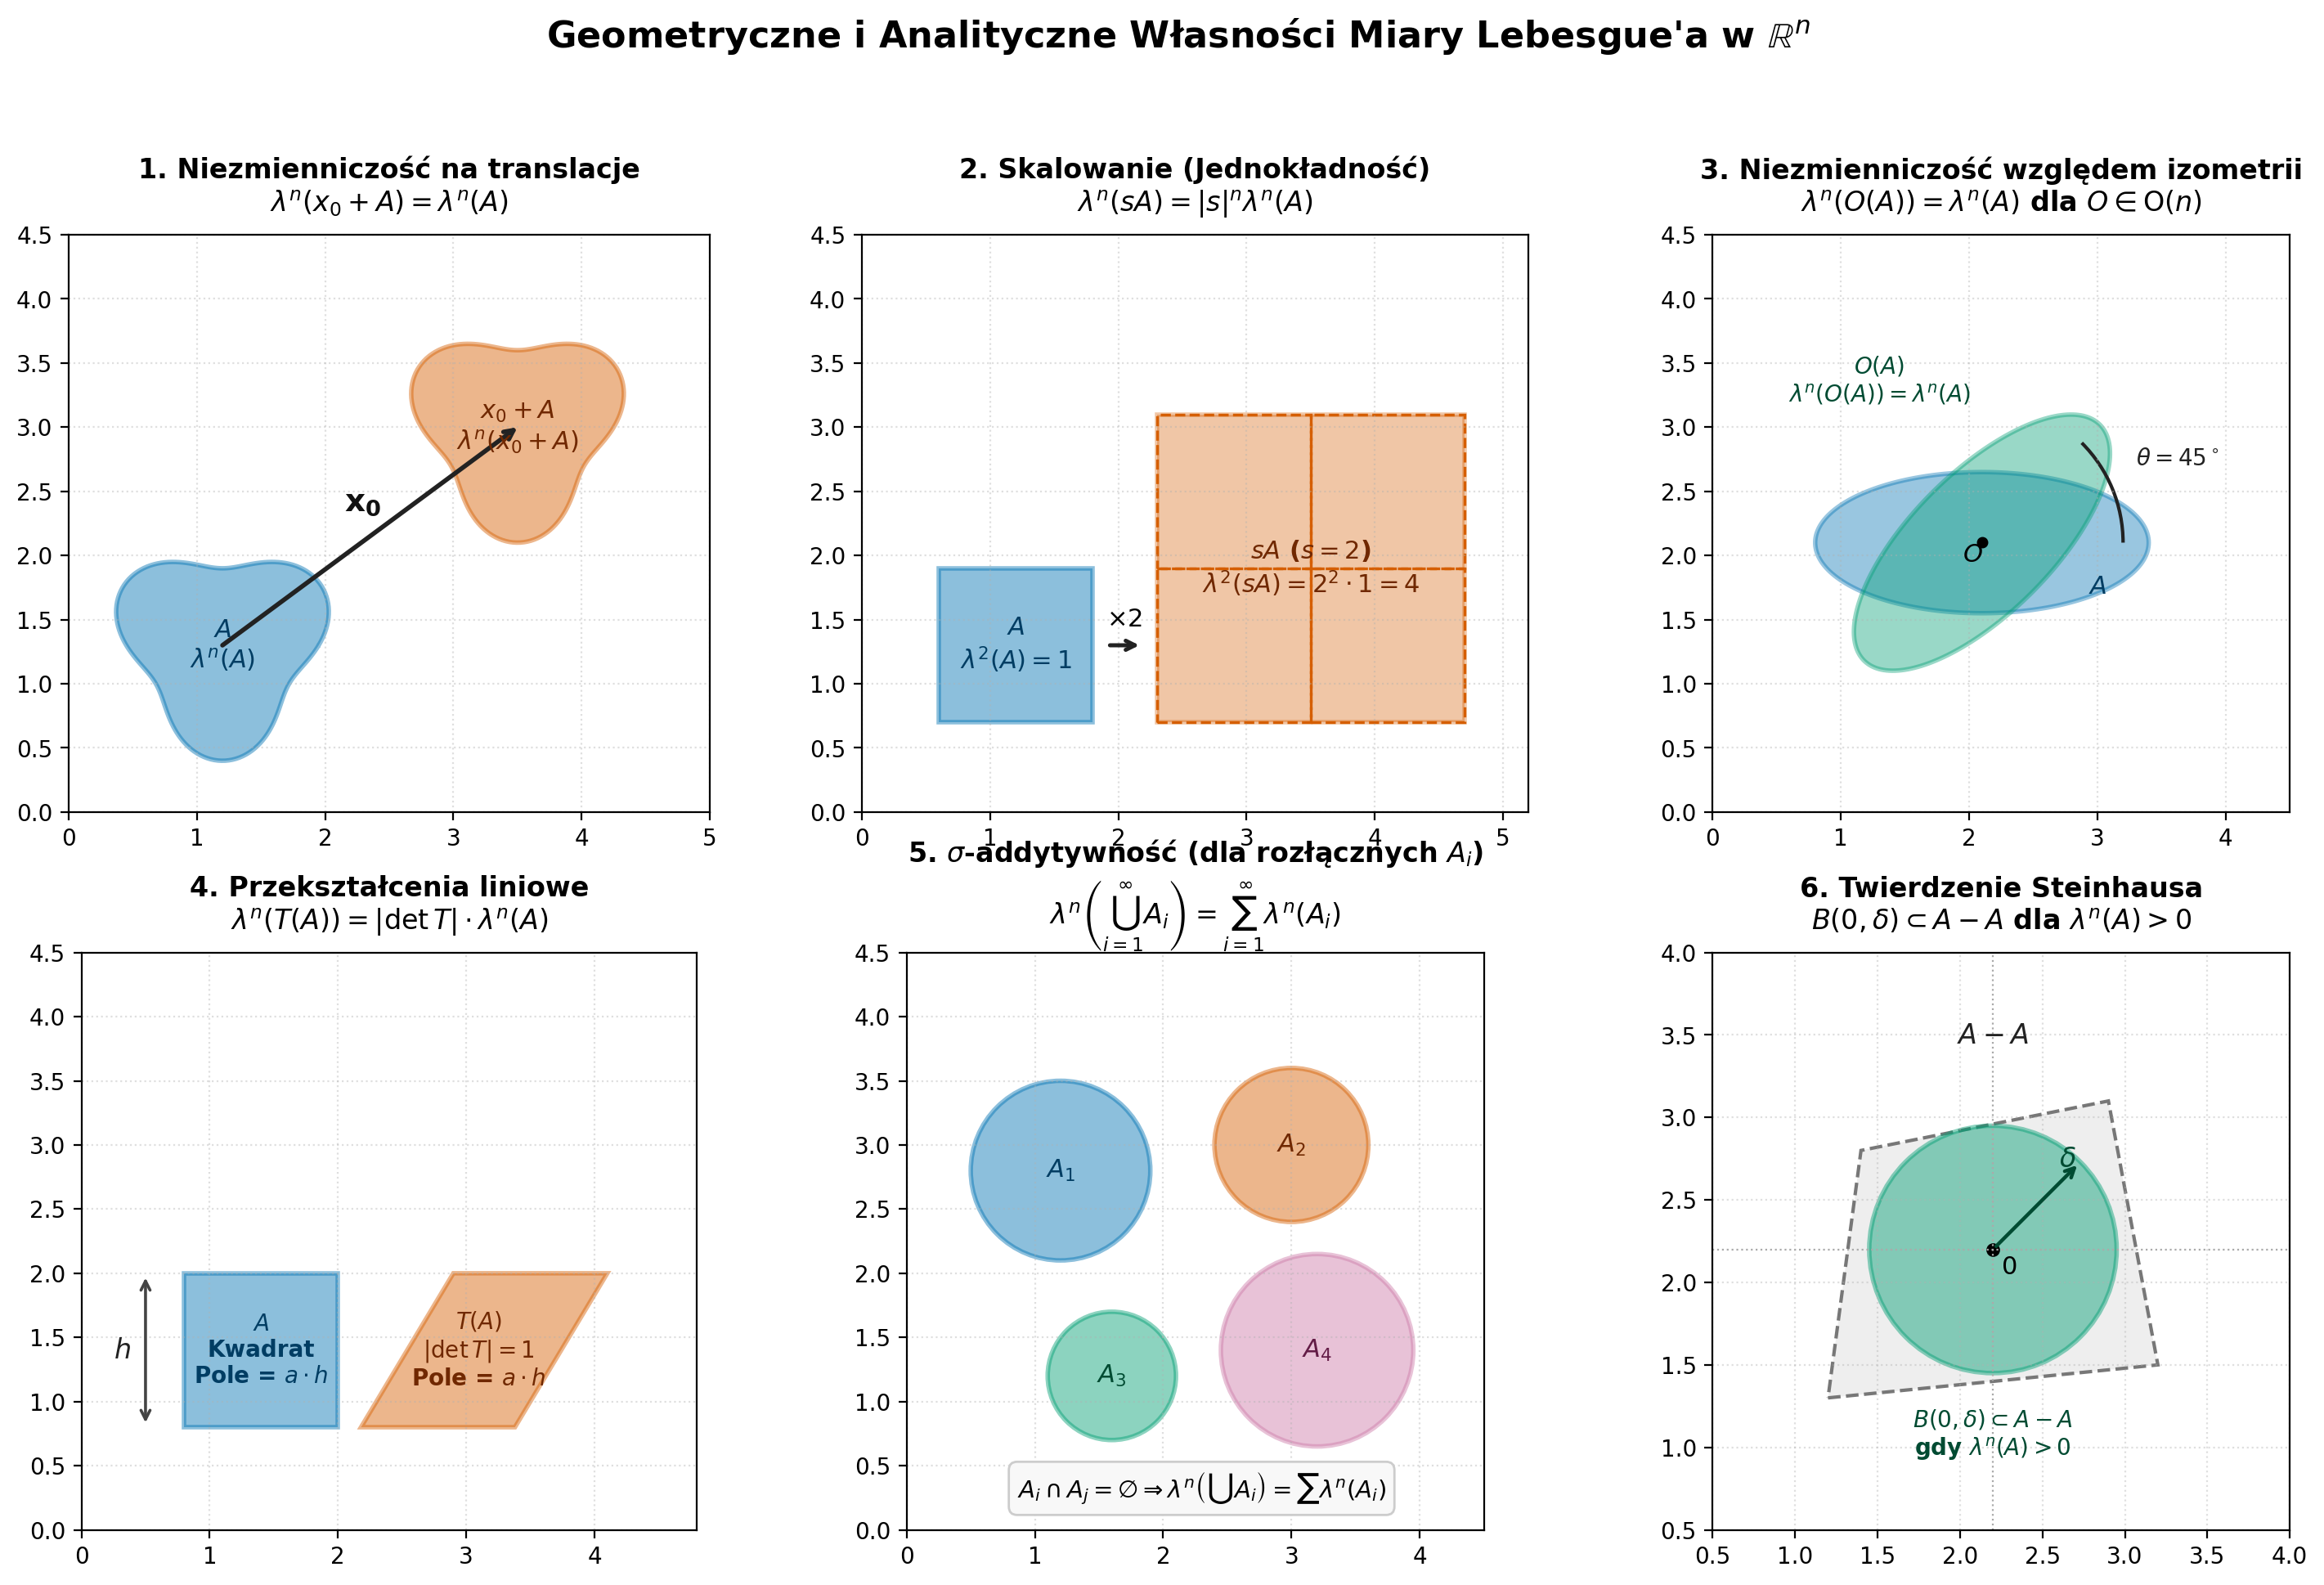
\includegraphics[width=0.95\textwidth]{wlasnosci_miary_lebesguea.png}
    \caption{Geometryczna interpretacja kluczowych własności miary Lebesgue'a w $\Rn$: translacji, skalowania, izometrii, przekształceń liniowych, $\sigma$-addytywności oraz twierdzenia Steinhausa.}
    \label{fig:wlasnosci_miary}
\end{figure}

\begin{tw}[Zachowanie miary przy translacji i skalowaniu]
    Niech $A \in \Leb{\Rn}$, $x_0 \in \Rn$ oraz $s \in \R$. Wówczas:
    \begin{enumerate}
        \item $x_0 + A \in \Leb{\Rn}$ oraz $\lambda^n(x_0 + A) = \lambda^n(A)$;
        \item $sA \in \Leb{\Rn}$ oraz $\lambda^n(sA) = |s|^n \lambda^n(A)$.
    \end{enumerate}
\end{tw}

\begin{tw}[Przekształcenia liniowe]\label{tw:transformacja_liniowa}
    Niech $T \colon \Rn \to \Rn$ będzie operatorem liniowym reprezentowanym przez macierz $M \in M_{n \times n}(\R)$. Jeżeli $A \in \Leb{\Rn}$, to $T(A) \in \Leb{\Rn}$ oraz:
    \begin{equation}
        \lambda^n(T(A)) = |\det T| \cdot \lambda^n(A).
    \end{equation}
\end{tw}

\begin{uwaga}[Intuicja geometryczna dla $n=2$]
    Pełny dowód pomijamy; wyjaśnimy jedynie, skąd bierze się czynnik $|\det T|$ (por.\ Rysunek~\ref{fig:wlasnosci_miary}). Każdą odwracalną macierz $2\times 2$ można zapisać jako złożenie trzech typów prostych przekształceń:
    \begin{enumerate}
        \item[(a)] \textbf{skalowania osi} $(x,y)\mapsto(ax,by)$: kwadrat jednostkowy przechodzi na prostokąt o bokach $|a|$ i $|b|$, więc pole mnoży się przez $|ab| = |\det T|$ (panel~2 rysunku);
        \item[(b)] \textbf{obrotu} (lub symetrii): figura jest przenoszona sztywno, pole się nie zmienia, a $|\det T| = 1$ (panel~3);
        \item[(c)] \textbf{ścinania} $(x,y)\mapsto(x+cy,\,y)$: kwadrat przechodzi na równoległobok o tej samej podstawie i tej samej wysokości, więc pole się nie zmienia, a $\det T = 1$ (panel~4).
    \end{enumerate}
    Ponieważ wyznacznik złożenia jest iloczynem wyznaczników, a pola mnożą się w ten sam sposób, dla każdego prostokąta $P$ otrzymujemy $\lambda^2(T(P)) = |\det T|\,\lambda^2(P)$; przybliżając dowolny zbiór mierzalny pokryciami prostokątami, dostajemy tę równość dla wszystkich $A \in \Leb{\R^2}$. Gdy $\det T = 0$, obraz $T(\R^2)$ jest prostą lub punktem, a więc zbiorem miary zero.
\end{uwaga}

\begin{wn}[Niezmienniczość względem izometrii]
    Każda izometria przestrzeni euklidesowej $\Phi \colon \Rn \to \Rn$ ma postać $\Phi(x) = Ox + x_0$, gdzie $O \in \mathrm{O}(n)$ jest macierzą ortogonalną ($O^T O = I$), a $x_0 \in \Rn$. Ponieważ $\det O = \pm 1$, dla każdego zbioru $A \in \Leb{\Rn}$ zachodzi:
    \begin{equation}
        \lambda^n(\Phi(A)) = |\det O| \cdot \lambda^n(A) = \lambda^n(A).
    \end{equation}
    W szczególności miara Lebesgue'a jest niezmiennicza na obroty wokół środka układu współrzędnych oraz symetrie zwierciadlane.
\end{wn}

\subsection{Własności strukturalne: bezatomowość i własność Darboux}

\begin{defi}[Atom miary]
    Niech $(X, \mathcal{M}, \mu)$ będzie przestrzenią z miarą. Zbiór $A \in \mathcal{M}$ o mierze $\mu(A) > 0$ nazywamy \textbf{atomem miary} $\mu$, jeżeli dla każdego podzbioru mierzalnego $B \in \mathcal{M}, B \subset A$ zachodzi:
    \begin{equation}
        \mu(B) = 0 \quad \text{albo} \quad \mu(B) = \mu(A).
    \end{equation}
    Miarę $\mu$ nazywamy \textbf{bezatomową}, jeżeli nie posiada ona żadnych atomów.
\end{defi}

\begin{tw}[Bezatomowość miary Lebesgue'a]
    Miara Lebesgue'a $\lambda^n$ w $\Rn$ jest miarą bezatomową.
\end{tw}

\begin{dow}
    Niech $A \in \Leb{\Rn}$ spełnia $\lambda^n(A) > 0$. Ponieważ $A = \bigcup_{m=1}^\infty \left(A \cap [-m, m]^n\right)$, z ciągłości miary z dołu istnieje $m \in \N$ takie, że zbiór $A_m := A \cap [-m, m]^n$ ma miarę $0 < \lambda^n(A_m) \mlr (2m)^n < +\infty$. Rozważmy półprzestrzenie $H_t = \{x \in \Rn \colon x_1 \mlr t\}$ dla $t \in \R$ i zdefiniujmy funkcję:
    \begin{equation*}
        f(t) := \lambda^n(A_m \cap H_t).
    \end{equation*}
    Funkcja $f$ jest niemalejąca, $f(t) = 0$ dla $t < -m$ oraz $f(t) = \lambda^n(A_m)$ dla $t \wlr m$. Ponadto $f$ jest ciągła, gdyż dla dowolnych $t_1 < t_2$:
    \begin{align*}
        0 \mlr f(t_2) - f(t_1) & = \lambda^n(A_m \cap \{x \colon t_1 < x_1 \mlr t_2\})                     \\
                               & \mlr \lambda^n\left([t_1, t_2] \times [-m, m]^{n-1}\right) = (2m)^{n-1}(t_2 - t_1).
    \end{align*}
    Z własności Darboux dla funkcji ciągłej $f$ istnieje punkt $t_0 \in \R$ taki, że:
    \begin{equation*}
        f(t_0) = \lambda^n(A_m \cap H_{t_0}) = \frac{1}{2} \lambda^n(A_m).
    \end{equation*}
    Kładąc $B = A_m \cap H_{t_0} \subset A$, otrzymujemy podzbiór mierzalny o mierze $0 < \lambda^n(B) = \frac{1}{2}\lambda^n(A_m) < \lambda^n(A_m) \mlr \lambda^n(A)$. Zbiór $A$ nie jest więc atomem, co dowodzi bezatomowości miary $\lambda^n$.
\end{dow}

\begin{wn}[Własność Darboux dla miary Lebesgue'a]
    Dla każdego zbioru mierzalnego $A \in \Leb{\Rn}$ oraz dowolnej liczby rzeczywistej $c$ spełniającej $0 \le c \le \lambda^n(A)$ istnieje zbiór mierzalny $B \subset A$ taki, że:
    \begin{equation}
        \lambda^n(B) = c.
    \end{equation}
\end{wn}

\begin{uwaga}[Twierdzenie Steinhausa]
    Dla zbioru $A \subset \Rn$ jego \textbf{zbiorem różnic} nazywamy zbiór $A - A := \{x - y \colon x, y \in A\}$. H.~Steinhaus udowodnił w 1920 roku, że jeżeli $A \in \Leb{\Rn}$ oraz $\lambda^n(A) > 0$, to zbiór $A - A$ zawiera pewną kulę otwartą $B(0, \delta)$, $\delta > 0$. Z twierdzenia tego wynika alternatywny dowód niemierzalności zbioru Vitalego $V$ z Twierdzenia~\ref{tw:vitali}: gdyby $V$ był mierzalny, miałby dodatnią miarę, tymczasem $(V - V) \cap \Q = \{0\}$, więc $V - V$ nie zawiera żadnego przedziału.
\end{uwaga}

\section{Podsumowanie}

\subsection{Główne wnioski}

\begin{enumerate}
    \item \textbf{Przezwyciężenie ograniczeń miary Jordana}:
          miara Jordana, oparta na skończonych pokryciach, nie mierzy nawet tak prostych zbiorów jak $\Q \cap [0, 1]$. Przejście do przeliczalnych pokryć i $\sigma$-addytywności sprawia, że każdy zbiór przeliczalny ma miarę zero, a zbiory mierzalne tworzą $\sigma$-algebrę zawierającą $\BorelRn$.

    \item \textbf{Zupełność}:
          przestrzeń $(\Rn, \Leb{\Rn}, \lambda^n)$ jest zupełna, tzn.\ każdy podzbiór zbioru miary zero jest mierzalny; $\Leb{\Rn}$ jest uzupełnieniem $\BorelRn$.

    \item \textbf{Topologiczna natura mierzalności}:
          każdy zbiór mierzalny różni się od pewnego zbioru typu $G_\delta$ (oraz od pewnego zbioru typu $F_\sigma$) o zbiór miary zero, a jego miarę można przybliżać miarami zbiorów otwartych z zewnątrz i zwartych od wewnątrz.

    \item \textbf{Granice mierzalności}:
          zbiór Vitalego pokazuje, że przy aksjomacie wyboru nie istnieje nietrywialna, $\sigma$-addytywna i niezmiennicza na translacje miara określona na całym $\mathcal{P}(\Rn)$.
\end{enumerate}

\subsection{Znaczenie miary Lebesgue'a w analizie matematycznej}

Najważniejszą motywacją konstrukcji miary Lebesgue'a jest całka Lebesgue'a. W odróżnieniu od całki Riemanna, która dzieli dziedzinę funkcji na przedziały, całka Lebesgue'a dzieli zbiór wartości funkcji i mierzy przeciwobrazy otrzymanych przedziałów. Wymaga to, by te przeciwobrazy były zbiorami mierzalnymi, a im bogatsza jest klasa zbiorów mierzalnych, tym więcej funkcji można całkować. Przykładem jest funkcja Dirichleta, czyli funkcja charakterystyczna zbioru $\Q \cap [0,1]$: nie jest ona całkowalna w sensie Riemanna, natomiast jej całka Lebesgue'a istnieje i jest równa zeru, ponieważ zbiór liczb wymiernych ma miarę Lebesgue'a zero. Dzięki $\sigma$-addytywności miary całka Lebesgue'a spełnia też silne twierdzenia o przechodzeniu do granicy pod znakiem całki, których brakuje w teorii Riemanna.

Na tym fundamencie zbudowano dużą część współczesnej analizy: przestrzenie funkcji całkowalnych, w których zupełność miary przekłada się na zupełność przestrzeni, oraz analizę Fouriera, w której kluczową rolę odgrywa niezmienniczość miary Lebesgue'a względem translacji.

Teoria miary stała się również językiem rachunku prawdopodobieństwa. W 1933 roku A.~Kołmogorow zdefiniował prawdopodobieństwo jako miarę unormowaną na $\sigma$-algebrze zdarzeń, a miara Lebesgue'a na odcinku $[0,1]$ jest naturalnym modelem rozkładu jednostajnego.

\begin{thebibliography}{7}

    \bibitem{Hartman}
    {\sc S. Hartman, J. Mikusiński},
    \textit{Teoria Miary i Całki Lebesgue'a},
    Państwowe Wydawnictwa Naukowe, 1957
    %
    \bibitem{Muszynski}
    {\sc J. Muszyński},
    \textit{Teoria całki},
    Państwowe Wydawnictwa Naukowe, 1990

    \bibitem{Cohn}
    {\sc D. L. Cohn},
    \textit{Measure Theory}, Birkhauser, 1980.

    \bibitem{Czyz}
    {\sc R. Czyż},
    \textit{Teoria miary i całki}, Uniwersytet Jagielloński, Kraków, 2020.

    \bibitem{Plebanek}
    {\sc G. Plebanek},
    \textit{Miara i całka. Skrypt do wykładu}, Instytut Matematyczny Uniwersytetu Wrocławskiego, Wrocław, 2020.

\end{thebibliography}


\end{document}
